\documentclass[conference]{IEEEtran}
% The preceding line is only needed to identify funding in the first footnote. If that is unneeded, please comment it out.
\usepackage{cite}
\usepackage{amsmath,amssymb,amsfonts}
\usepackage{algorithmic}
\usepackage{graphicx}
\usepackage{textcomp}
\usepackage{xcolor}
\usepackage[acronym]{glossaries}
\usepackage{subcaption}
\usepackage[flushleft]{threeparttable}
\usepackage{booktabs}
\usepackage{adjustbox}
\usepackage{enumitem}
\usepackage{float}


\usepackage{hyperref}
\usepackage{multirow}
\newcommand{\STAB}[1]{\begin{tabular}{@{}c@{}}#1\end{tabular}}

\setlist{parsep=0pt,listparindent=\parindent}

\def\BibTeX{{\rm B\kern-.05em{\sc i\kern-.025em b}\kern-.08em
    T\kern-.1667em\lower.7ex\hbox{E}\kern-.125emX}}
\begin{document}
\title{Object detection for Verification Based Annotation}
\author{\IEEEauthorblockN{Oliver Batchelor\IEEEauthorrefmark{1} and
Richard Green\IEEEauthorrefmark{2}}
\IEEEauthorblockA{Department of Computer Science,
University of Canterbury\\
Christchurch, New Zealand\\
Email: \IEEEauthorrefmark{1}oliver.batchelor@canterbury.ac.nz,
\IEEEauthorrefmark{2}richard.green@canterbury.ac.nz}}


\newacronym{VBA}{VBA}{Verification Based Annotation}
\newacronym{FCN}{FCN}{Fully Convolutional Network}
\newacronym{FPN}{FPN}{Feature Pyramid Network}


\newacronym{IID}{IID}{Independent and Identically Distributed}

\newacronym{IOU}{IoU}{Intersection over Union}
\newacronym{VOC}{VOC}{Visual Object Classes}
\newacronym{mIOU}{mIOU}{mean Intersection Over Union}

\newacronym{mAP}{mAP}{mean Average Precision}
\newacronym{AP}{AP}{Average Precision}


\newacronym{CRF}{CRF}{Conditional Random Field}

\newacronym{RELU}{ReLU}{Rectified Linear Unit}
\newacronym{PRELU}{PReLU}{Parameterised Rectified Linear Unit}
\newacronym{DECAF}{DeCAF}{Deep Convolutional Activation Feature}

\newacronym{FPN}{FPN}{Feature Pyramid Network}


\newacronym{NLL}{NLL}{Negative Loss Likelihood}
\newacronym{BCE}{BCE}{Binary Cross Entropy}
\newacronym{CE}{CE}{Cross Entropy}

\newacronym{EER}{EER}{Equal Error Rate}

 
\newacronym{COCO}{COCO}{Microsoft Common Objects in Context}
\newacronym{ILSVRC}{ILSVRC}{ImageNet Large Scale Visual Recognition Challenge}

\newacronym{NN}{NN}{Neural Network}
\newacronym{DNN}{DNN}{Deep Neural Network}

\newacronym{CNN}{CNN}{Convolutional Neural Network}
\newacronym{MCDNN}{MCDNN}{Multi-Column Deep Neural Network}

\newacronym{SSD}{SSD}{Single Shot Detector}
\newacronym{RCNN}{R-CNN}{Region CNN}

\newacronym{NMS}{NMS}{ Non-Maxima Suppression}


\newacronym{SIFT}{SIFT}{Scale Invariant Feature Transform}
\newacronym{SURF}{SURF}{Speeded Up Robust Features}

\newacronym{ALOI}{ALOI}{Amsterdam Library of Images}
\newacronym{MSR}{MSR}{Microsoft Research}
\newacronym{AMT}{AMT}{Amazon Mechanical Turk}

\newacronym{BOW}{BoW}{Bag of Words}
\newacronym{BOVW}{BoVW}{Bag of Visual Words}

\newacronym{ANN}{ANN}{Approximate Nearest Neighbour}
\newacronym{SGD}{SGD}{Stochastic Gradient Descent}
\newacronym{ASGD}{ASGD}{Asynchronous Stochastic Gradient Descent}
\newacronym{LOO}{LOO}{Leave One Out}

\newacronym{NCA}{NCA}{Neighbourhood Components Analysis}
\newacronym{MEGM}{MEGM}{Mean square Error's Gradient Minimisation}

\newacronym{KNN}{kNN}{k-Nearest Neighbour}

\newacronym{MSE}{MSE}{Mean Squared Error}
\newacronym{LMNN}{LMNN}{Large Margin Nearest Neighbour}
\newacronym{NCM}{NCM}{Nearest Class Mean}

\newacronym{SVM}{SVM}{Support Vector Machine}

\newacronym{PCA}{PCA}{Principle Components Analysis}
\newacronym{DRLIM}{DrLIM}{Dimensionality Reduction by Learning an Invariant Mapping}
\newacronym{SGDR}{SGDR}{Stochastic Gradient Descent with Restarts}


\newacronym{GPU}{GPU}{Graphics Processing Unit} 
\newacronym{CPU}{CPU}{Central Processing Unit}

\newacronym{API}{API}{Application Programming Interface} 

\newacronym{GHC}{GHC}{Glasgow Haskell Compiler}
\newacronym{GHCJS}{GHCJS}{GHC for JavaScript}

\newacronym{HTML}{HTML}{HyperText Markup Language}
\newacronym{SVG}{SVG}{Scaleable Vector Graphics}

\newacronym{HTTP}{HTTP}{HyperText Transfer Protocol}
\newacronym{JSON}{JSON}{JavaScript Object Notation}

\newacronym{ID}{ID}{Index of Difficulty}
\newacronym{AWS}{AWS}{Amazon Web Services}

\newacronym{CAT}{CAT}{Cumulative Annotation Time}
\newacronym{ROV}{ROV}{Remotely Operated Vehicle}


\maketitle

\begin{abstract}


In this paper, we examine the properties of an object detector for Verification Based Annotation (VBA), where annotation is performed by having machine annotations checked and verified (and corrected, in this work) by a human annotator. We show that with a few modifications from standard practice, a convolutional neural network based object detector can be a robust aid to annotation, without a large degree of parameter tweaking. We previously annotated a variety of small-scale datasets which we attempt to validate some of our ideas and assumptions for an object detector used for VBA.

Our approach is to use high-resolution images, training on image crops (as opposed to the usual practice of resizing input images to a fixed resolution), and find this method successful, being more accurate and robust than down-scaling. A particular interest is the effect of localisation noise and systematic bias in annotations. We characterise the impact on object detection performance and compare to human levels, we find noise has a large impact, especially with fewer training examples.

\end{abstract}

\begin{IEEEkeywords}
verification, annotation, object detection, neural network, human-in-the-loop
\end{IEEEkeywords}

\section{Introduction}

\begin{figure*}[htb]
\centering
\begin{subfigure}[t]{0.2\linewidth}
  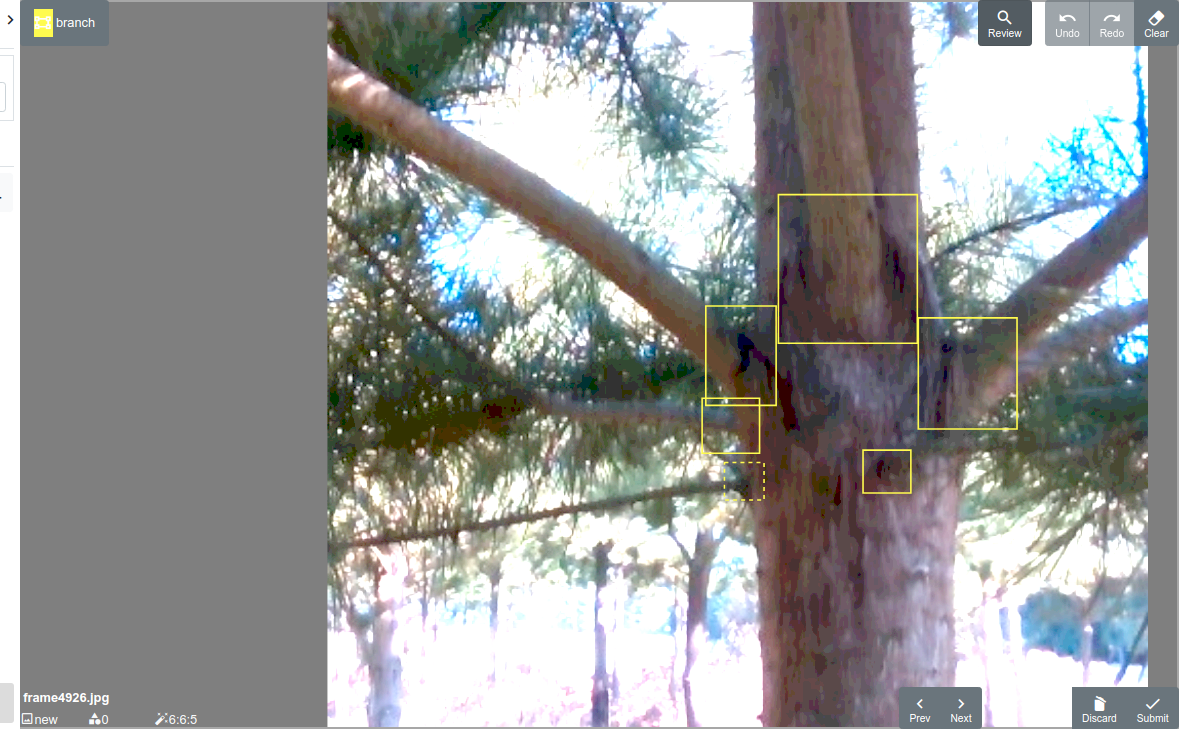
\includegraphics[width=0.9\linewidth]{figures/images/branches3.png}
   \caption{\emph{branches}}
\end{subfigure}%
\begin{subfigure}[t]{0.2\linewidth}
  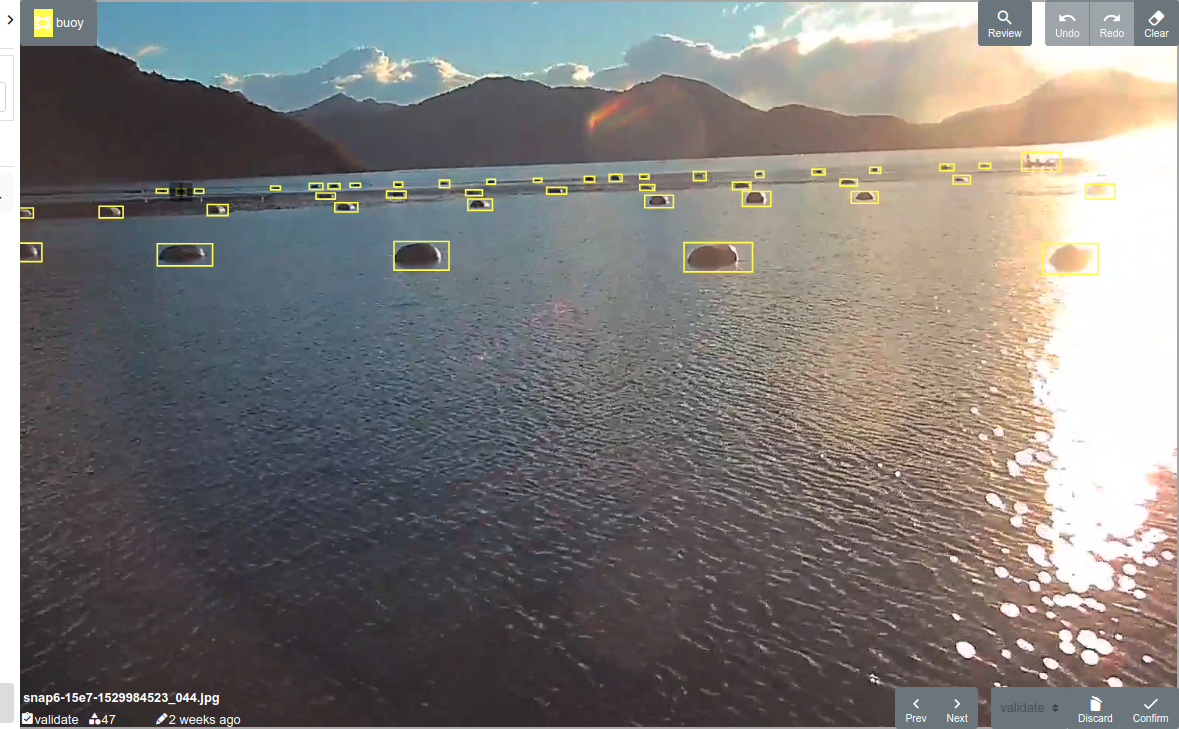
\includegraphics[width=0.9\linewidth]{figures/images/buoys.png}
   \caption{\emph{buoys}}
 \end{subfigure}%
\begin{subfigure}[t]{0.2\linewidth}
  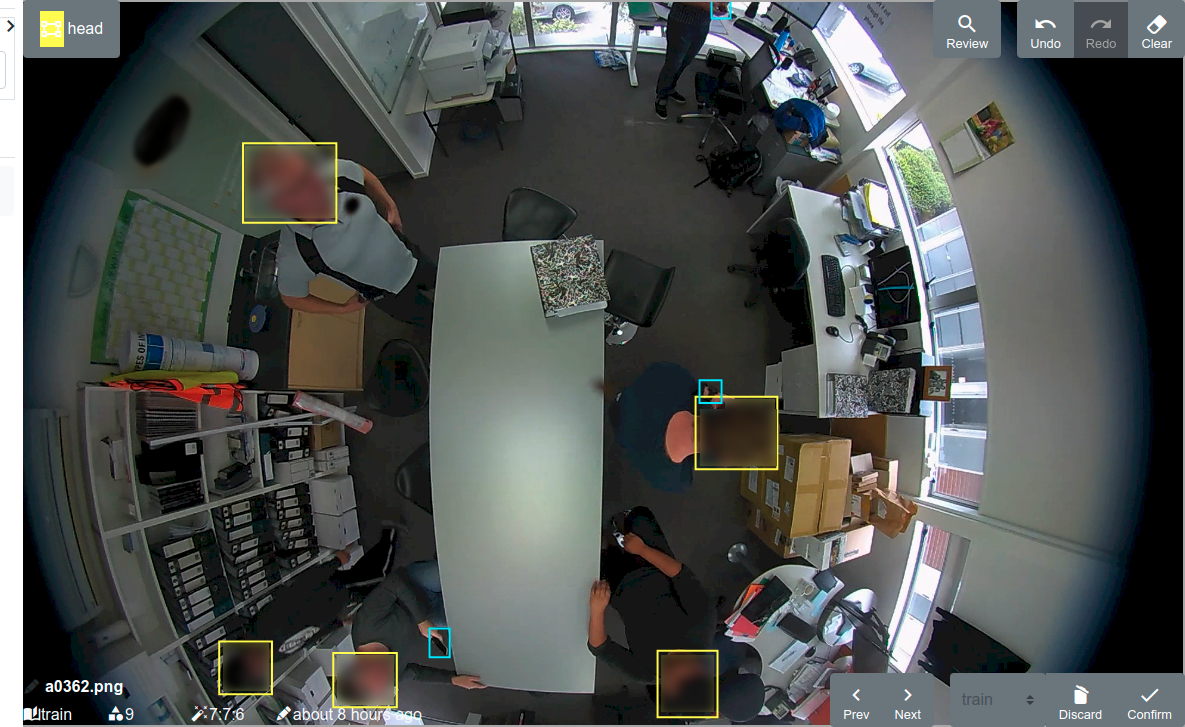
\includegraphics[width=0.9\linewidth]{figures/images/victor.png}
  \caption{\emph{fisheye}}
\end{subfigure}%
\begin{subfigure}[t]{0.2\linewidth}
  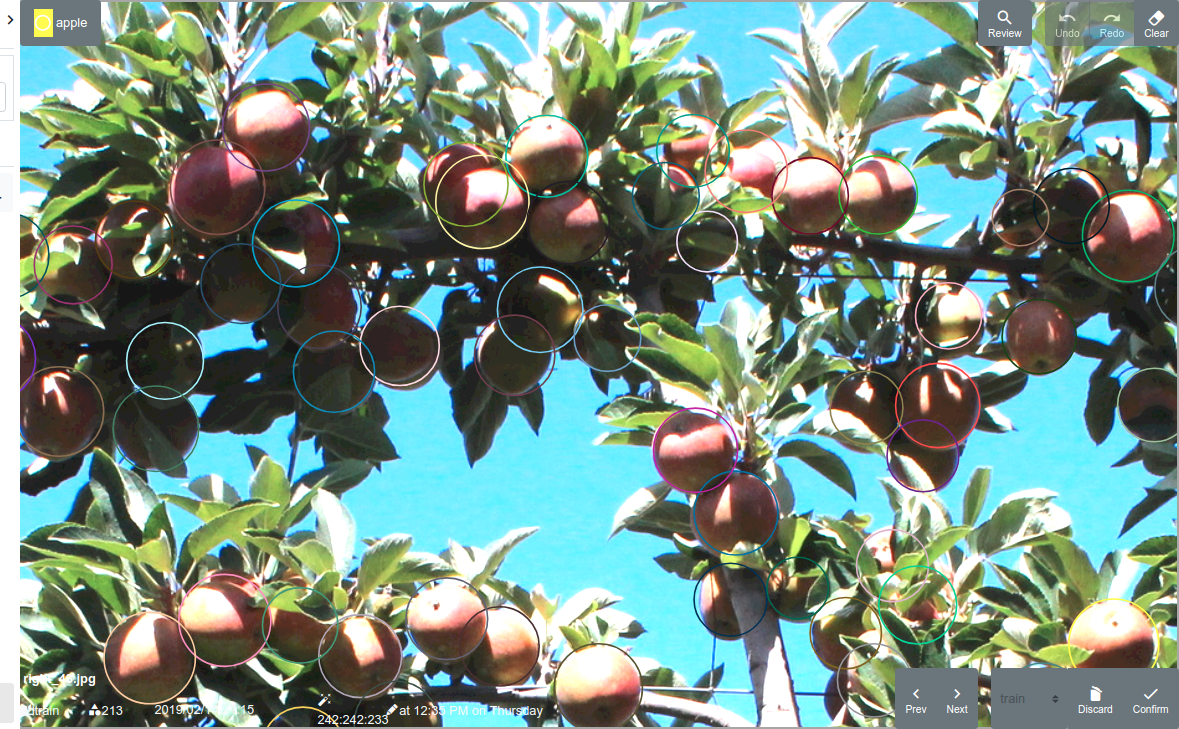
\includegraphics[width=0.9\linewidth]{figures/images/apples_big2.png}
  \caption{$\mathrm{apples_1}$}
\end{subfigure}%
\begin{subfigure}[t]{0.2\linewidth}
  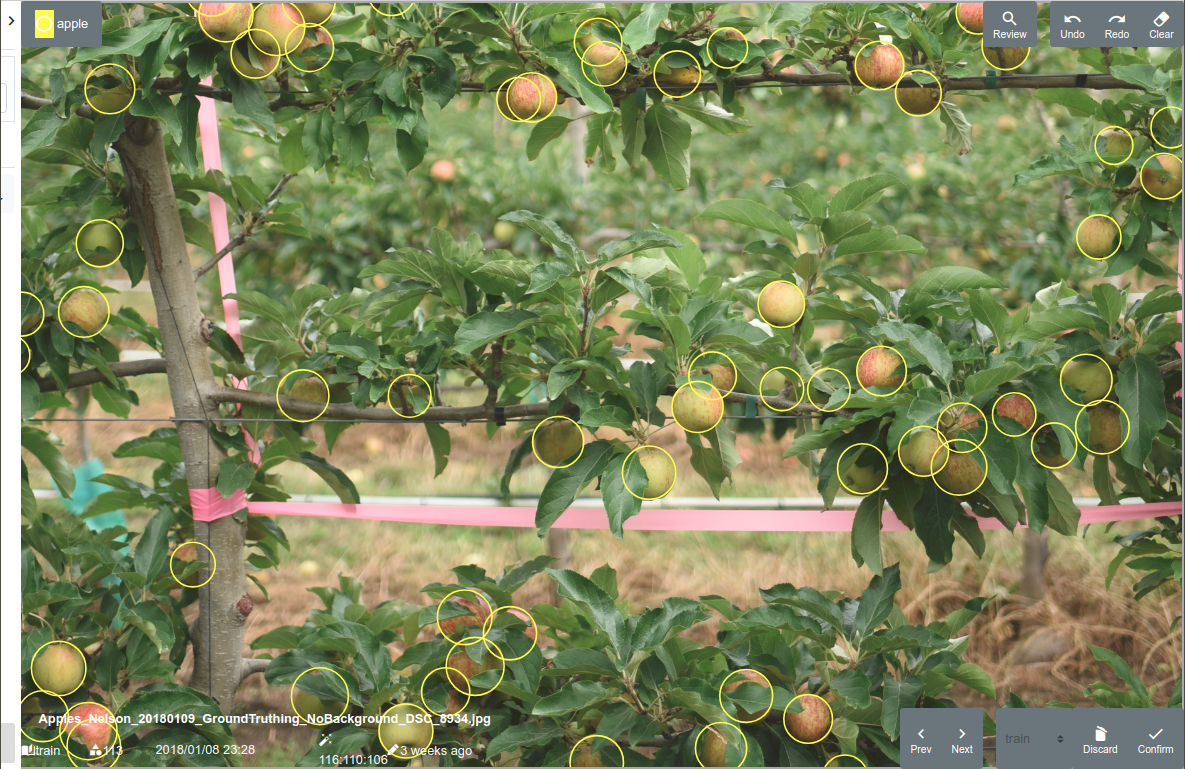
\includegraphics[width=0.9\linewidth]{figures/images/apples2.png}
  \caption{$\mathrm{apples_2}$}
\end{subfigure}
\begin{subfigure}[t]{0.2\linewidth}
  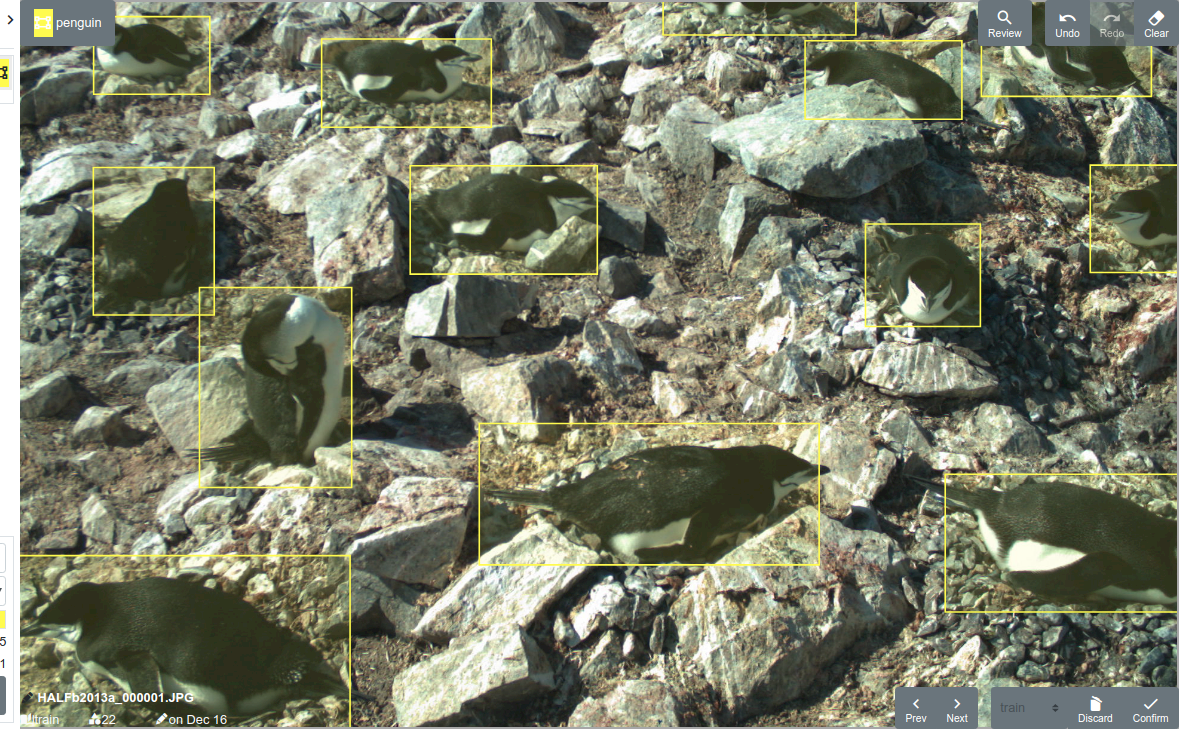
\includegraphics[width=0.9\linewidth]{figures/images/penguins2.png}
   \caption{\emph{penguins}}
\end{subfigure}%
 \begin{subfigure}[t]{0.2\linewidth}
  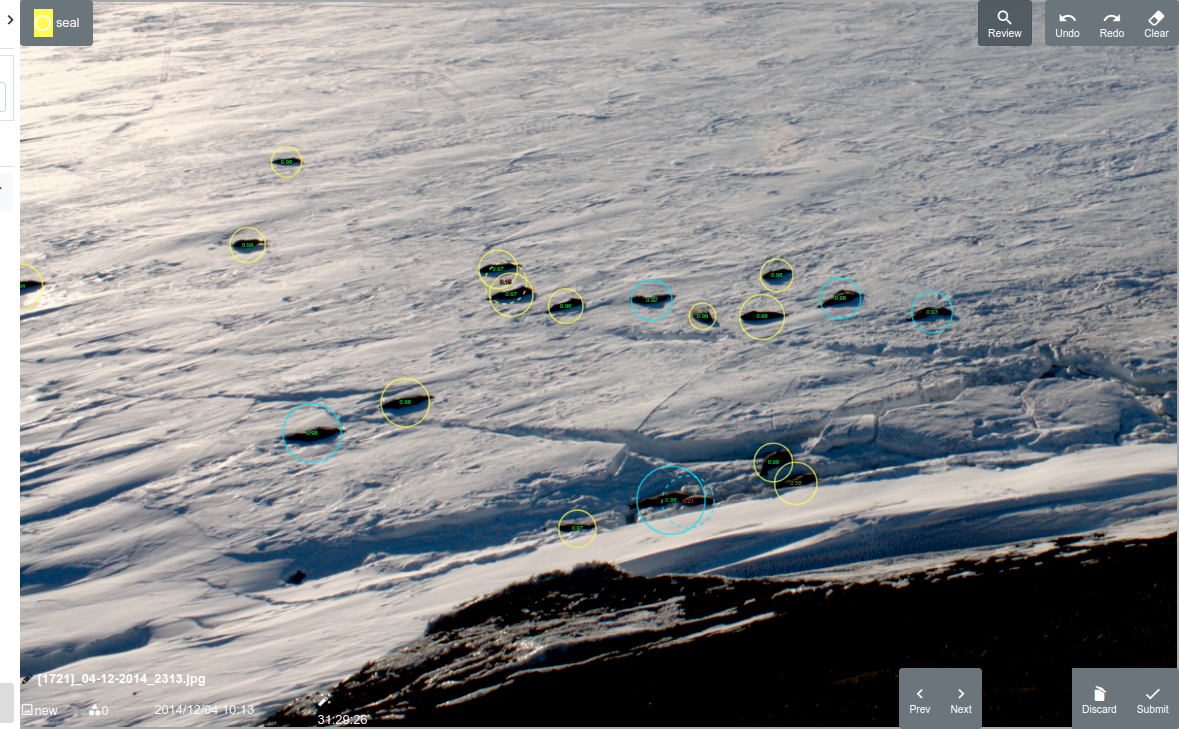
\includegraphics[width=0.9\linewidth]{figures/images/seals_small2.png}
  \caption{\emph{seals}}
\end{subfigure}%
\begin{subfigure}[t]{0.2\linewidth}
  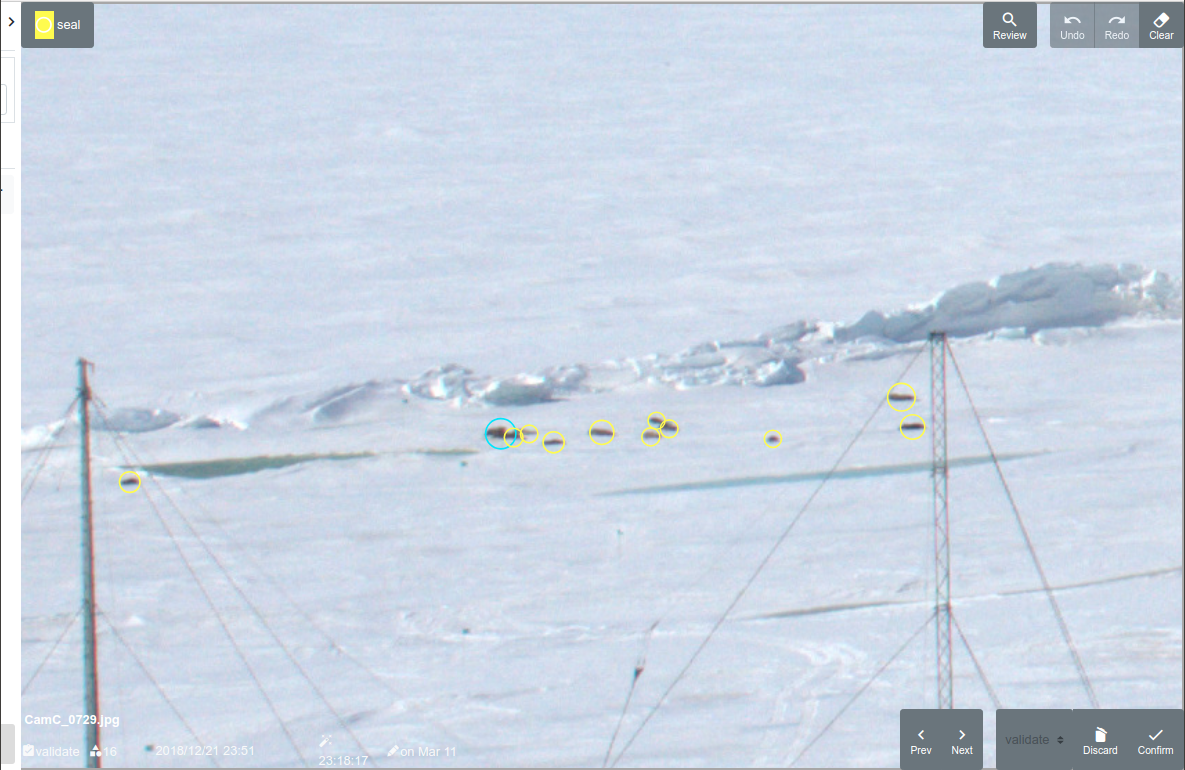
\includegraphics[width=0.9\linewidth]{figures/images/scott_base_sunny.png}
  \caption{\emph{scott base}}
\end{subfigure}%
\begin{subfigure}[t]{0.2\linewidth}
  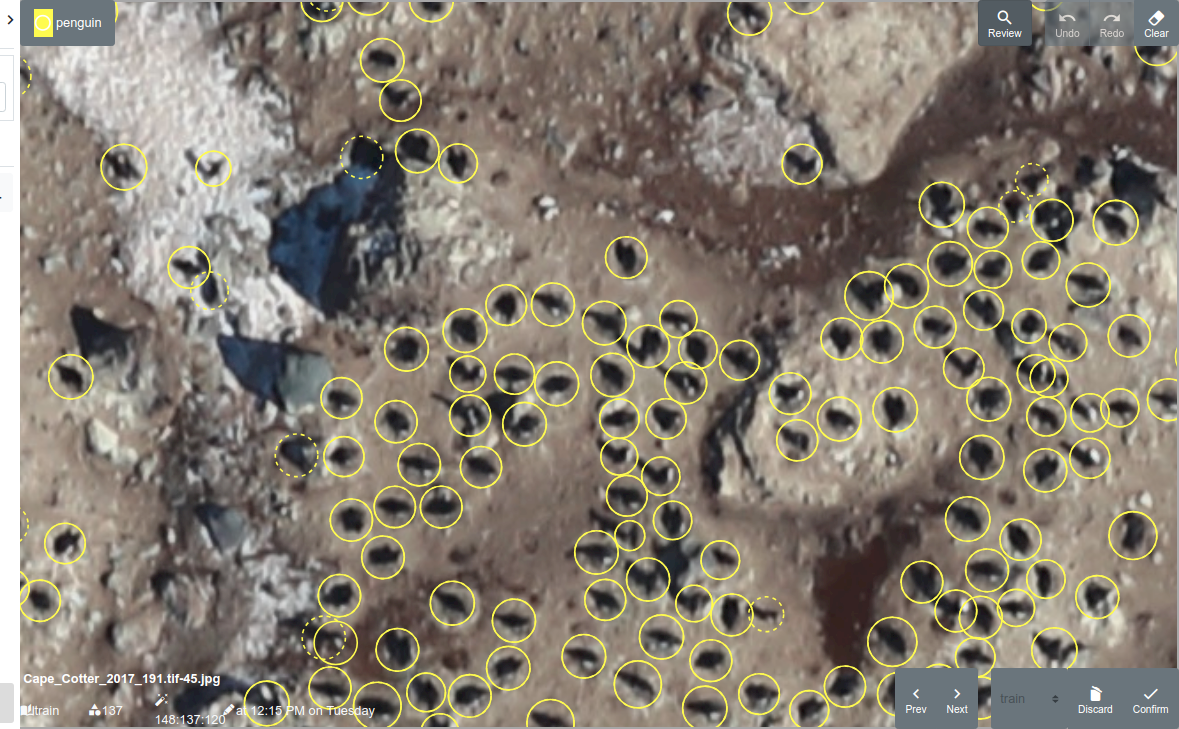
\includegraphics[width=0.9\linewidth]{figures/images/penguins_aerial2.png}
  \caption{\emph{penguin survey}}
\end{subfigure}%
\begin{subfigure}[t]{0.2\linewidth}
  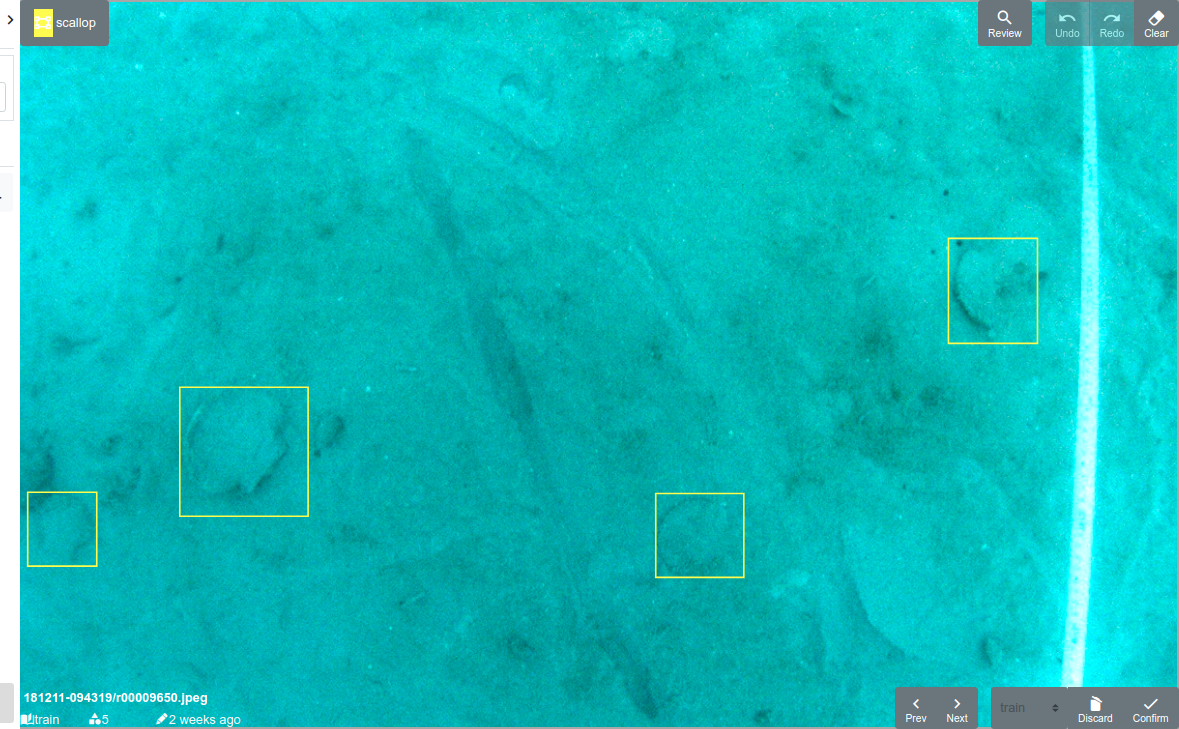
\includegraphics[width=0.9\linewidth]{figures/images/scallops4.png}
  \caption{\emph{scallops}}
\end{subfigure}
\caption{Representative images of datasets (and annotations) annotated in this work}
\label{fig:datasets_all}
\end{figure*}

Verification Based Annotation (VBA) is a form of \emph{Human-in-the-loop} machine learning, a collaboration between machine and human.  Human-in-the-loop approaches can offer improved engagement in activities that would otherwise be a laborious task. In \gls{VBA} algorithms machine annotations are verified by a human annotator, examples include question answering \cite{Papadopoulos2016}, semi-automatic segmentation \cite{Castrejon2017}, or as in this work modifying machine predictions \cite{Yao2012, Russakovsky2015a, McNeill2011}. 

In this paper, we examine the properties of an object detector used as part of a \gls{VBA} process. We are most interested in the robustness to varying parameters, such as image size, number and size of objects, and to initialisation. The ability to learn incrementally is key (and in particular, learn from a minimal number of examples). 


\subsection{Verification Based Annotation}

\gls{VBA} is a form of \emph{Human-in-the-loop} machine learning, a collaboration between a machine learning algorithm and a human user. The goal, where it relates to image annotation, is to make the most effective use of annotator time and reduce cognitive load.

Verification also plays a large part in ensuring consistency between human annotators in crowdsourcing efforts \cite{Su2012a}. The annotations of any one user cannot be fully trusted, and there can be significant variation between annotators. Often large organisations gamify the annotation process by having users annotate and verify labels as part of a proof-of-human process \cite{von2008recaptcha}.

Weaker algorithms (machine learning or otherwise) can be used to generate proposals which can then be validated by an annotator. An example of this is in \cite{McNeill2011} where computer vision algorithms generate proposed counts of a penguin colony, and a human operator marks false negatives and false positives.

Human verification is fast; in \cite{Papadopoulos2016}, a yes/no verification is reported as taking 1.6 seconds on average. For a full annotation of a \gls{ILSVRC} image, in \cite{Su2012a} the time to draw a bounding box is reported at 26 seconds (42 seconds after quality control), but \cite{Papadopoulos2017} reports only 7 seconds per box using a more effective input method involving clicking extremities of objects rather than selecting corners. 

\section {Setup and Method}
\subsection {Object detection}


\begin{table*}[thb]
\centering
\begin{threeparttable}
\centering
\caption{Overview of datasets, showing the variety in image and object size and number.  } 
\label{tab:resolutions} 
\begin{tabular}{l|lllllll}
dataset & annotations & images & box length & image size & train crop & $AP_{COCO}$ & automated \\
\toprule
$penguins$        & 7473        & 306    & $255 \pm 118$   &  $2048\times1536$  & 800                                   & 75.9  & 82.6\%                 \\
$branches$        & 2249        & 451    & $41.5 \pm 13.9$ &  $400\times400$    & 320                                   & 62.6  & 76.8\%                  \\
$seals$           & 4351        & 240    & $68.7 \pm 20.8$ &  $3920\times1600$  & 1024                                    & 80.7   & 93.4\%                 \\
$seals_b$         & 1256        & 82     & $63.4 \pm 17$   & $3920\times1600$  & 1024                                    & 72.9  & 87.3\%       \\
$scott\:base$     & 7759        & 301    & $15 \pm 3.21$     & $3927\times500$ -- $5200\times700$ & 400  & 81.4 & 84.8\%  \\
$apples^1$        & 21637       & 300    & $78.4 \pm 14.9$ &  $2592\times1728$ & 1024 & 51.8   & 75.1\%                  \\
$apples^2$        & 13418       & 168    & $92.8 \pm 11.9$ &  $3008\times2008$  & 1024                                    & 74.5  & 76.1\%                 \\
$scallops_e$      & 3669        & 6741   & $114 \pm 40.2$  &  $1280\times1024$  & 800                                   & 65.0    & 62.3\%               \\
$fisheye$         & 2598        & 367    & $96.6 \pm 32.7$ &  $2048\times1944$ & 1024                                     & 78.9   & 91.8\%                  \\
$buoys_d$         & 7221        & 207    & $38.9 \pm 42.8$ &  $1920\times1080$ & 600                                    & 70.9      & 89.9\%               \\
$penguin\:survey$ & 13210       & 352    & $22.6 \pm 2.11$ & $406\times405$ -- $672\times448$ & 400  & 61.6  & 89.5\%            \\ 
\bottomrule
\end{tabular}
\begin{tablenotes}
\small
\item Subscripts denote different annotators.  Datasets specified without subscript are annotated by the authors. $AP_{COCO}$ is measured on the split validation set. Box length is the length of the longest side (or diameter for circle annotations). Automated is the total proportion of annotations created from object detections without edit.

\end{tablenotes}
\end{threeparttable}
\end{table*}

The object detector is based on a single-shot \gls{CNN} detector called RetinaNet \cite{Lin2017}, an anchor-box based single stage object detector. This detector was selected for its simplicity and efficiency while having close to state-of-the-art accuracy. Some modifications from the method in \cite{Lin2017} and brief motivations for each are:

\begin{itemize}
    \item {\textbf {Sharing}}: no shared weights between classification sub-networks at different pyramid levels, to make training much faster at the beginning.
    \item {\textbf {Non normalised loss}}:
    We do not normalise of the loss function (by the number of anchor matches), to accommodate images with no positive annotations.
    \item {\textbf {High resolution}}: We train on crops of high-resolution images, but for inference operate on complete images. The motivation is to make the object detection task as easy as possible; larger objects are easier to detect \cite{Lin2014}. 
    \item {\textbf {Cyclical learning rates}}: We use of cyclical learning rates in training, to accommodate incremental additions to the training set.
    \item {\textbf{Extra decoder layers}}: We used an extra residual block at each resolution to combine shortcut connections after concatenation with features from lower resolutions.
\end{itemize}

We test some of the hypotheses which led to these decisions. Additionally, we present a study on how localisation noise and systematic error impacts training. The tolerance to localisation error (as well as the ability of the object detector to accurately localise objects) is crucial to how efficient a \gls{VBA} system can be.

\subsection{Metrics}

We use \gls{AP} at different levels of \gls{IOU} threshold for evaluation. This is the \gls{AP} across all examples and not a \gls{mAP} (largely academic because most datasets here are single class). This is notated $AP_{t}$ for \gls{IOU} threshold $t$. In particular two thresholds we use are $AP_{50}$ for a relaxed matching threshold and $AP_{75}$ for a strict threshold and then $AP_{COCO}$ for an average over a range of thresholds. $AP_{COCO}$ is defined as the mean of $AP_t$ for $t \in [0.5, 0.55..0.95]$.

\subsection{Training parameters}

In all experiments in this work I use a \gls{SGD} optimiser with the base learning rate set to $0.001$, momentum $0.9$ and weight decay $0.0001$ in all cases. Total loss is averaged across each mini-batch, and batch sizes of $8$ are used. The balance factor between localisation and classification loss is $\lambda=2.5$ in all cases. A cyclical learning rate is used during over each batch, with a log interpolated (geometric) multiplier reducing the learning rate by a factor of $0.1$ at the end of the batch. 

Image augmentation is used, crops taken at varied scale (${3/4}$--${4/3}$) and aspect ratio ($\pm 10\%$), flips ($0.5$ probability). A range of photo-metric augmentations: brightness ($\pm 10\%$), contrast ($\pm 10\%$), gamma adjustment ($\pm 0.1\%$), hue ($\pm 5$) and saturation ($\pm 5$) adjustment.

Code for this paper can be found \href{https://github.com/saulzar/detection/tree/thesis}{link}, under the tag ``thesis'', with details surrounding the cropping procedure, default training and augmentation parameters etc.

\subsection{Datasets}

A selection of images of the datasets and typical annotations used in this paper can be seen in Figure~\ref{fig:datasets_all} and a summary of the different variations can be seen in Table~\ref{tab:resolutions}, most of the datasets were annotated by the author, a few annotated by third parties and one was annotated by both. The datasets span a wide variety of image resolutions, and object sizes; the images in some cases are reduced resolution from the captured images, in other cases reducing the resolution would make object detection impossible.

A selection of the datasets with images and annotations (as well as annotation history logs) can be found at \href{http://academictorrents.com/details/e780e1a9e898e53e72c16cb5fcc6d61d90cc4d27}{link}. 


\section{High resolution inference}

We looked at two different possibilities for performing inference on a full-resolution image using an object detector network trained only on crops of images: (a) pass in the full image using the property that the network is \emph{fully convolutional} and (b) tile images the same size as training crops and collapse the predictions using a combined \gls{NMS}. To facilitate this idea, the box annotations on the edge of images are estimates of the full bounds of the object, and the anchor boxes are not cropped to the edge of the image. 

The first method is to pass in the full image to the neural network, even though it has only been trained on much smaller crops. Object detection networks are flexible and work across a range of input image resolutions. All layers are either convolutions or do not reshape the feature maps (aside from up/down-sampling). Passing in a larger image results in a larger feature map and set of box outputs at each layer of the pyramid. 

The second inference method is to tile multiple inferences at the size the model was trained at, across the full image size a overlap buffer region. The result is sets of overlapping predictions at the edges which be decimated using \gls{NMS}. 

Image size has its limits for both training and inference, as the complexity of the model and the size of the memory on the \gls{GPU} determines the maximum size image which can be processed. We can process the large images used in this work because of the relatively simple backbone model used (ResNet-18 \cite{He}). Evaluation using tiling makes it feasible to use larger image sizes and more complicated models, even if multiple inferences take more time.


\subsection {Effect of image resolution and crop size}
\label{sec:scale_crop}

For this experiment we vary the scale and crop size to test the idea that a high-resolution object detector can be trained on small parts of images, then the whole image used in inference.

\begin{figure*}[htb]
 \begin{subfigure}[t]{0.5\linewidth}
  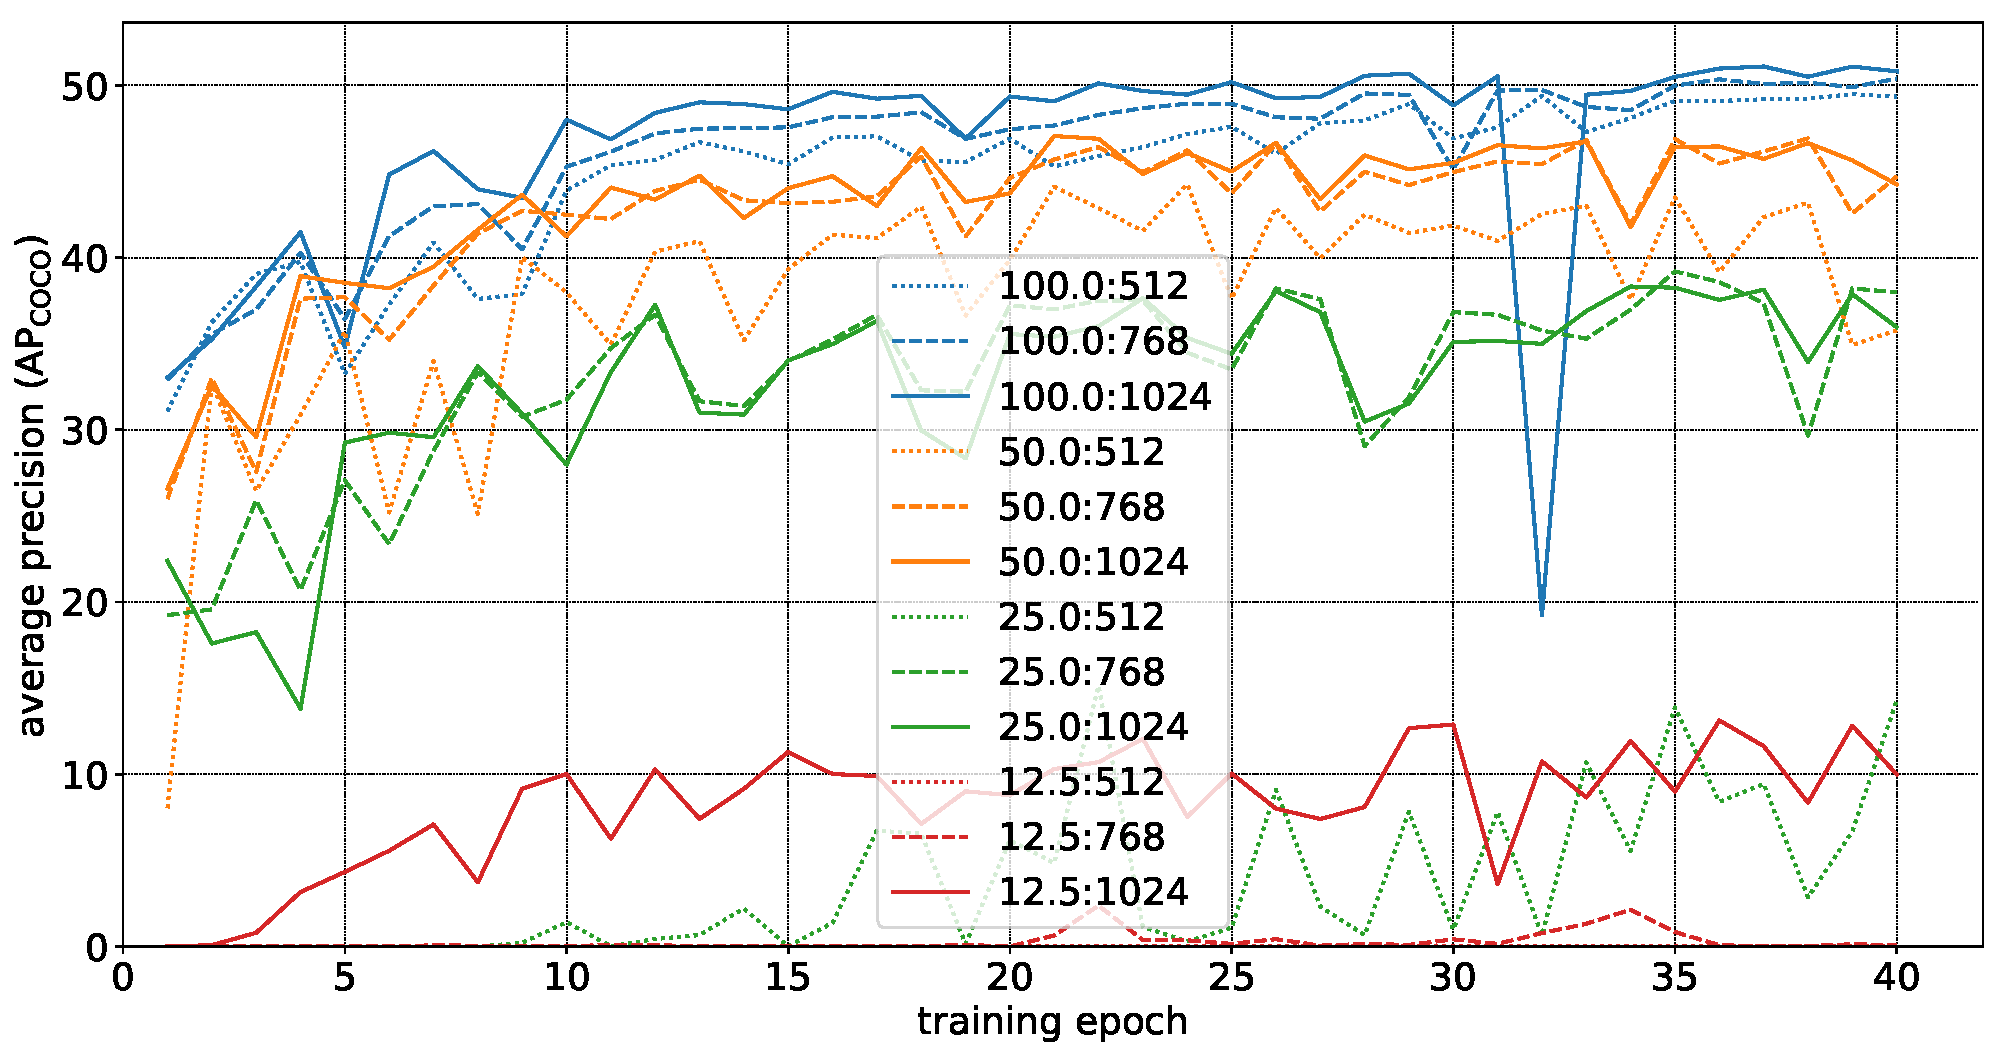
\includegraphics[width=1.0\linewidth]{figures/crops_scales/apples.pdf}
  \label{fig:apples_crop_scale}
\end{subfigure}%
 \begin{subfigure}[t]{0.5\linewidth}
  \centering
  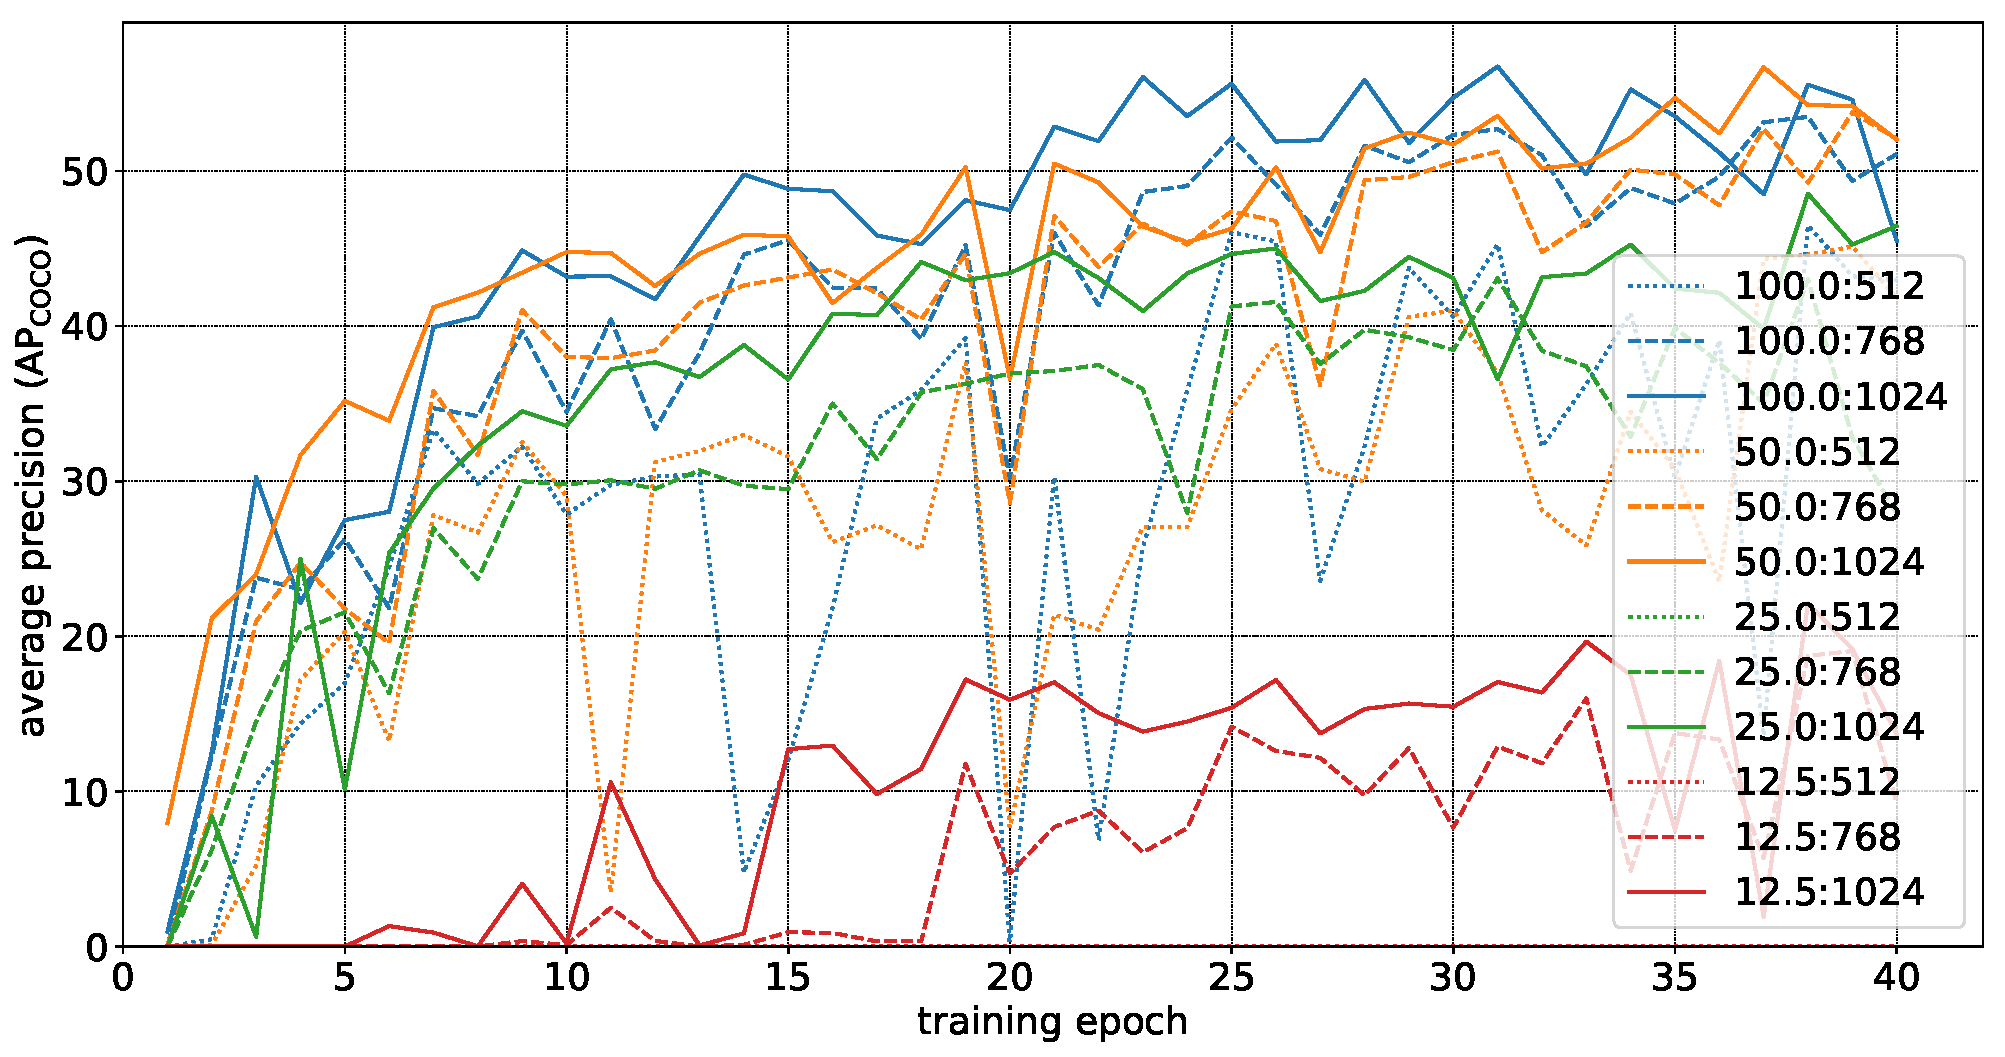
\includegraphics[width=1.0\linewidth]{figures/crops_scales/scallops.pdf}
  \label{fig:seals_crop_scale}  
\end{subfigure}%
  \caption{Comparison training at different crop sizes and scales for (a) $apples^1$ and (b) \emph{scallops} dataset. Crop size is presented as the crop size in the original image, the crop used for training is scaled by the given factor. } 
\end{figure*}
  


\begin{table}[h!]
  \centering
    \caption{Effect of scale and crop size on validation accuracy (percent of best $AP_{COCO}$). Average across datasets ($apples^1$, \emph{penguins}, \emph{scallops}, \emph{seals}) }
    
  \begin{tabular}{ l l | l l l l}
    & scale & 12.5\% & 25\% & 50\% & 100\% \\
    \toprule
       \multirow{2}{*}{\STAB{\rotatebox[origin=c]{90}{crop}}}
       & 512   & 0.0  & 2.4  &  59.3  & 82.8 \\
       & 768   & 17.4 & 68.2  &  90.0 &  96.4 \\
       & 1024  & 28.5 & 81.9  &  95.0  & 100.0 \\
    \bottomrule
  \end{tabular}
\label{tab:accuracy_scale_crop}
\end{table}

Using a larger crop size proved more accurate in all of the four datasets, and using a larger crop was beneficial in all cases, being more accurate and more stable to train. The larger size, however, trains much more slowly. In this case a factor of $3.3$ slower for half scale or half-size crop, larger factors having less speedup due to constants such as loading the images. Despite the relatively low requirement for fast inference (to keep up with a single annotator); this could be used for example for image selection, to find images of most uncertainty for active learning.

\subsection {Inference method for large images}

\begin{figure}[htb] 
  \centering
  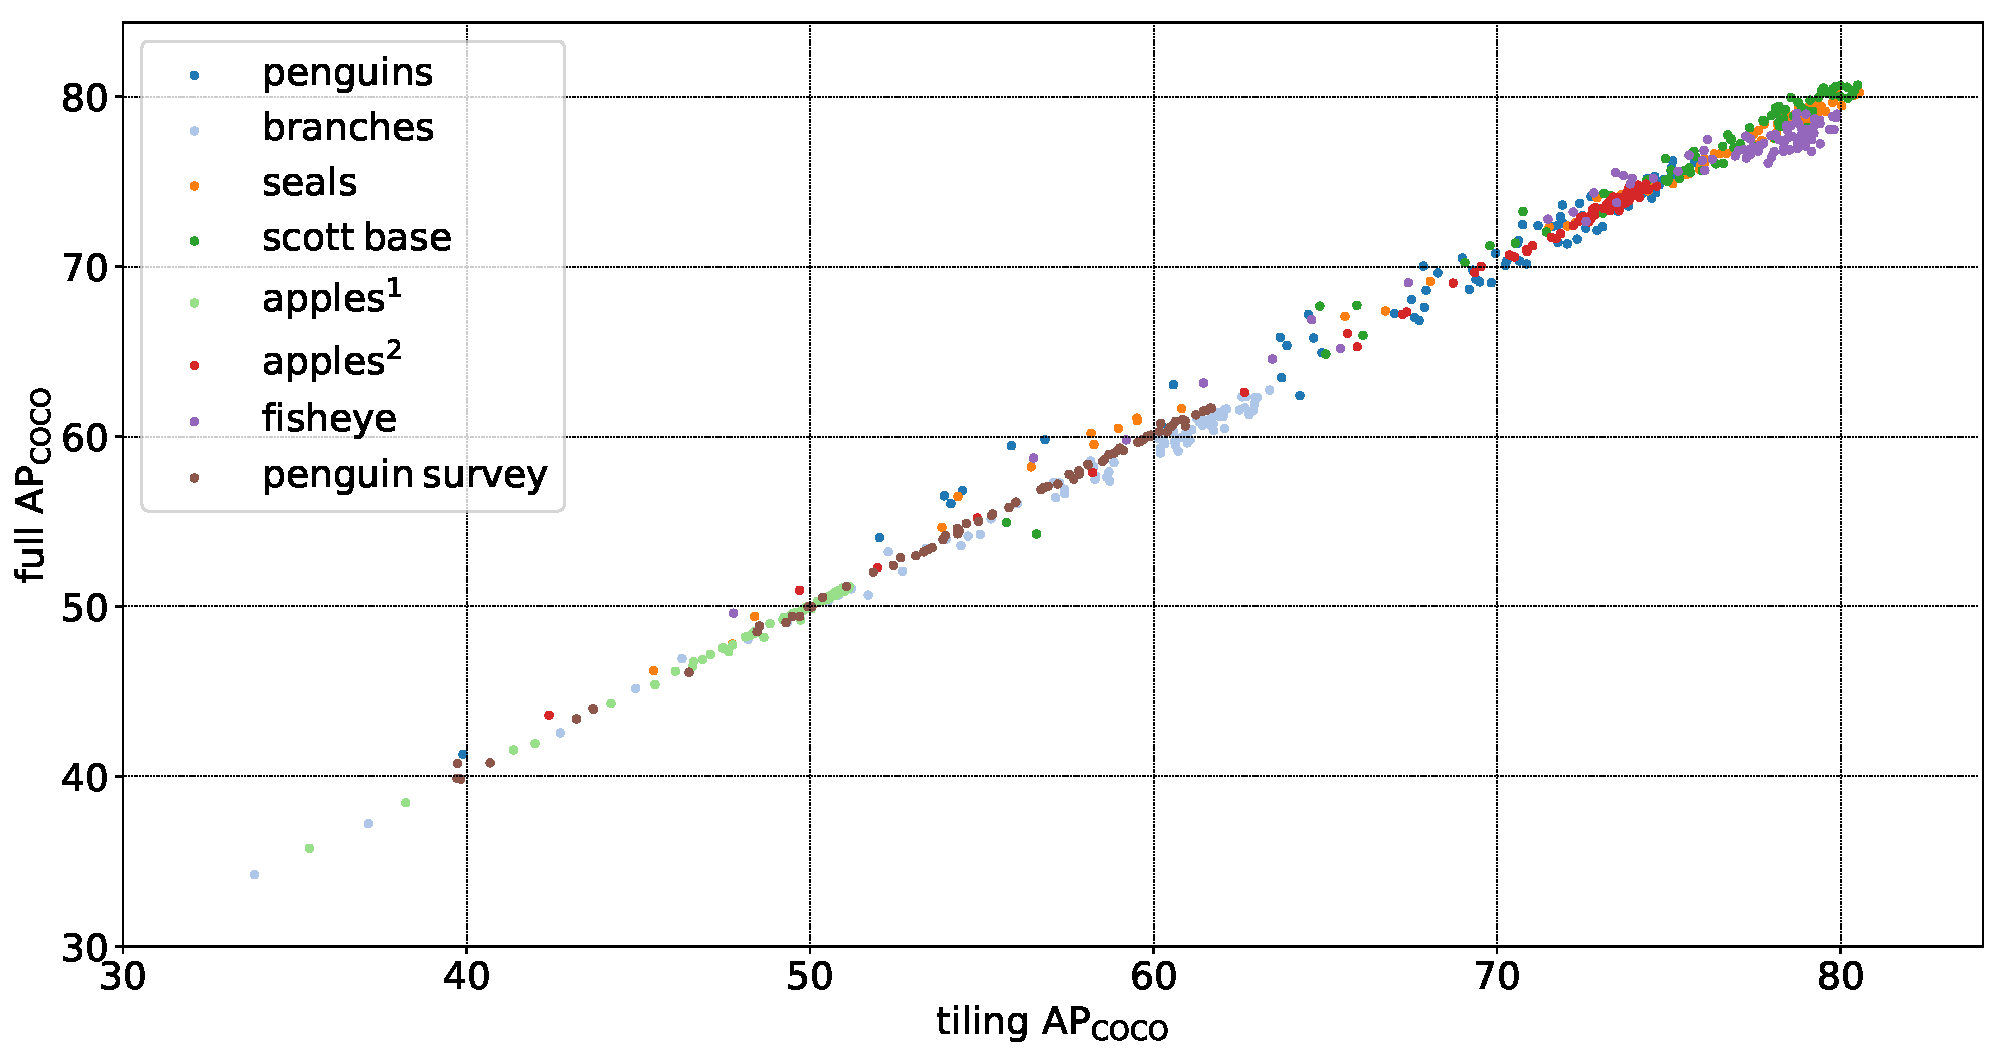
\includegraphics[width=1.0\linewidth]{figures/splits_scatters.pdf}
  \caption{Comparison of different inference methods across one training run with inference using tiling vs. Inference on full images. Training occurs on crops and evaluating on full images. }   
  \label{fig:inference_method}
\end{figure}


We compared the two methods (tiling vs inference on the full image) by using both methods for testing against the validation set of several different training runs. It can be seen in figure \ref{fig:inference_method} that both perform very similarly. Sometimes one is marginally better, and sometimes the other is marginally better, even within the same training run.



\section {Incremental training}

\begin{figure}[ht]
  \centering
  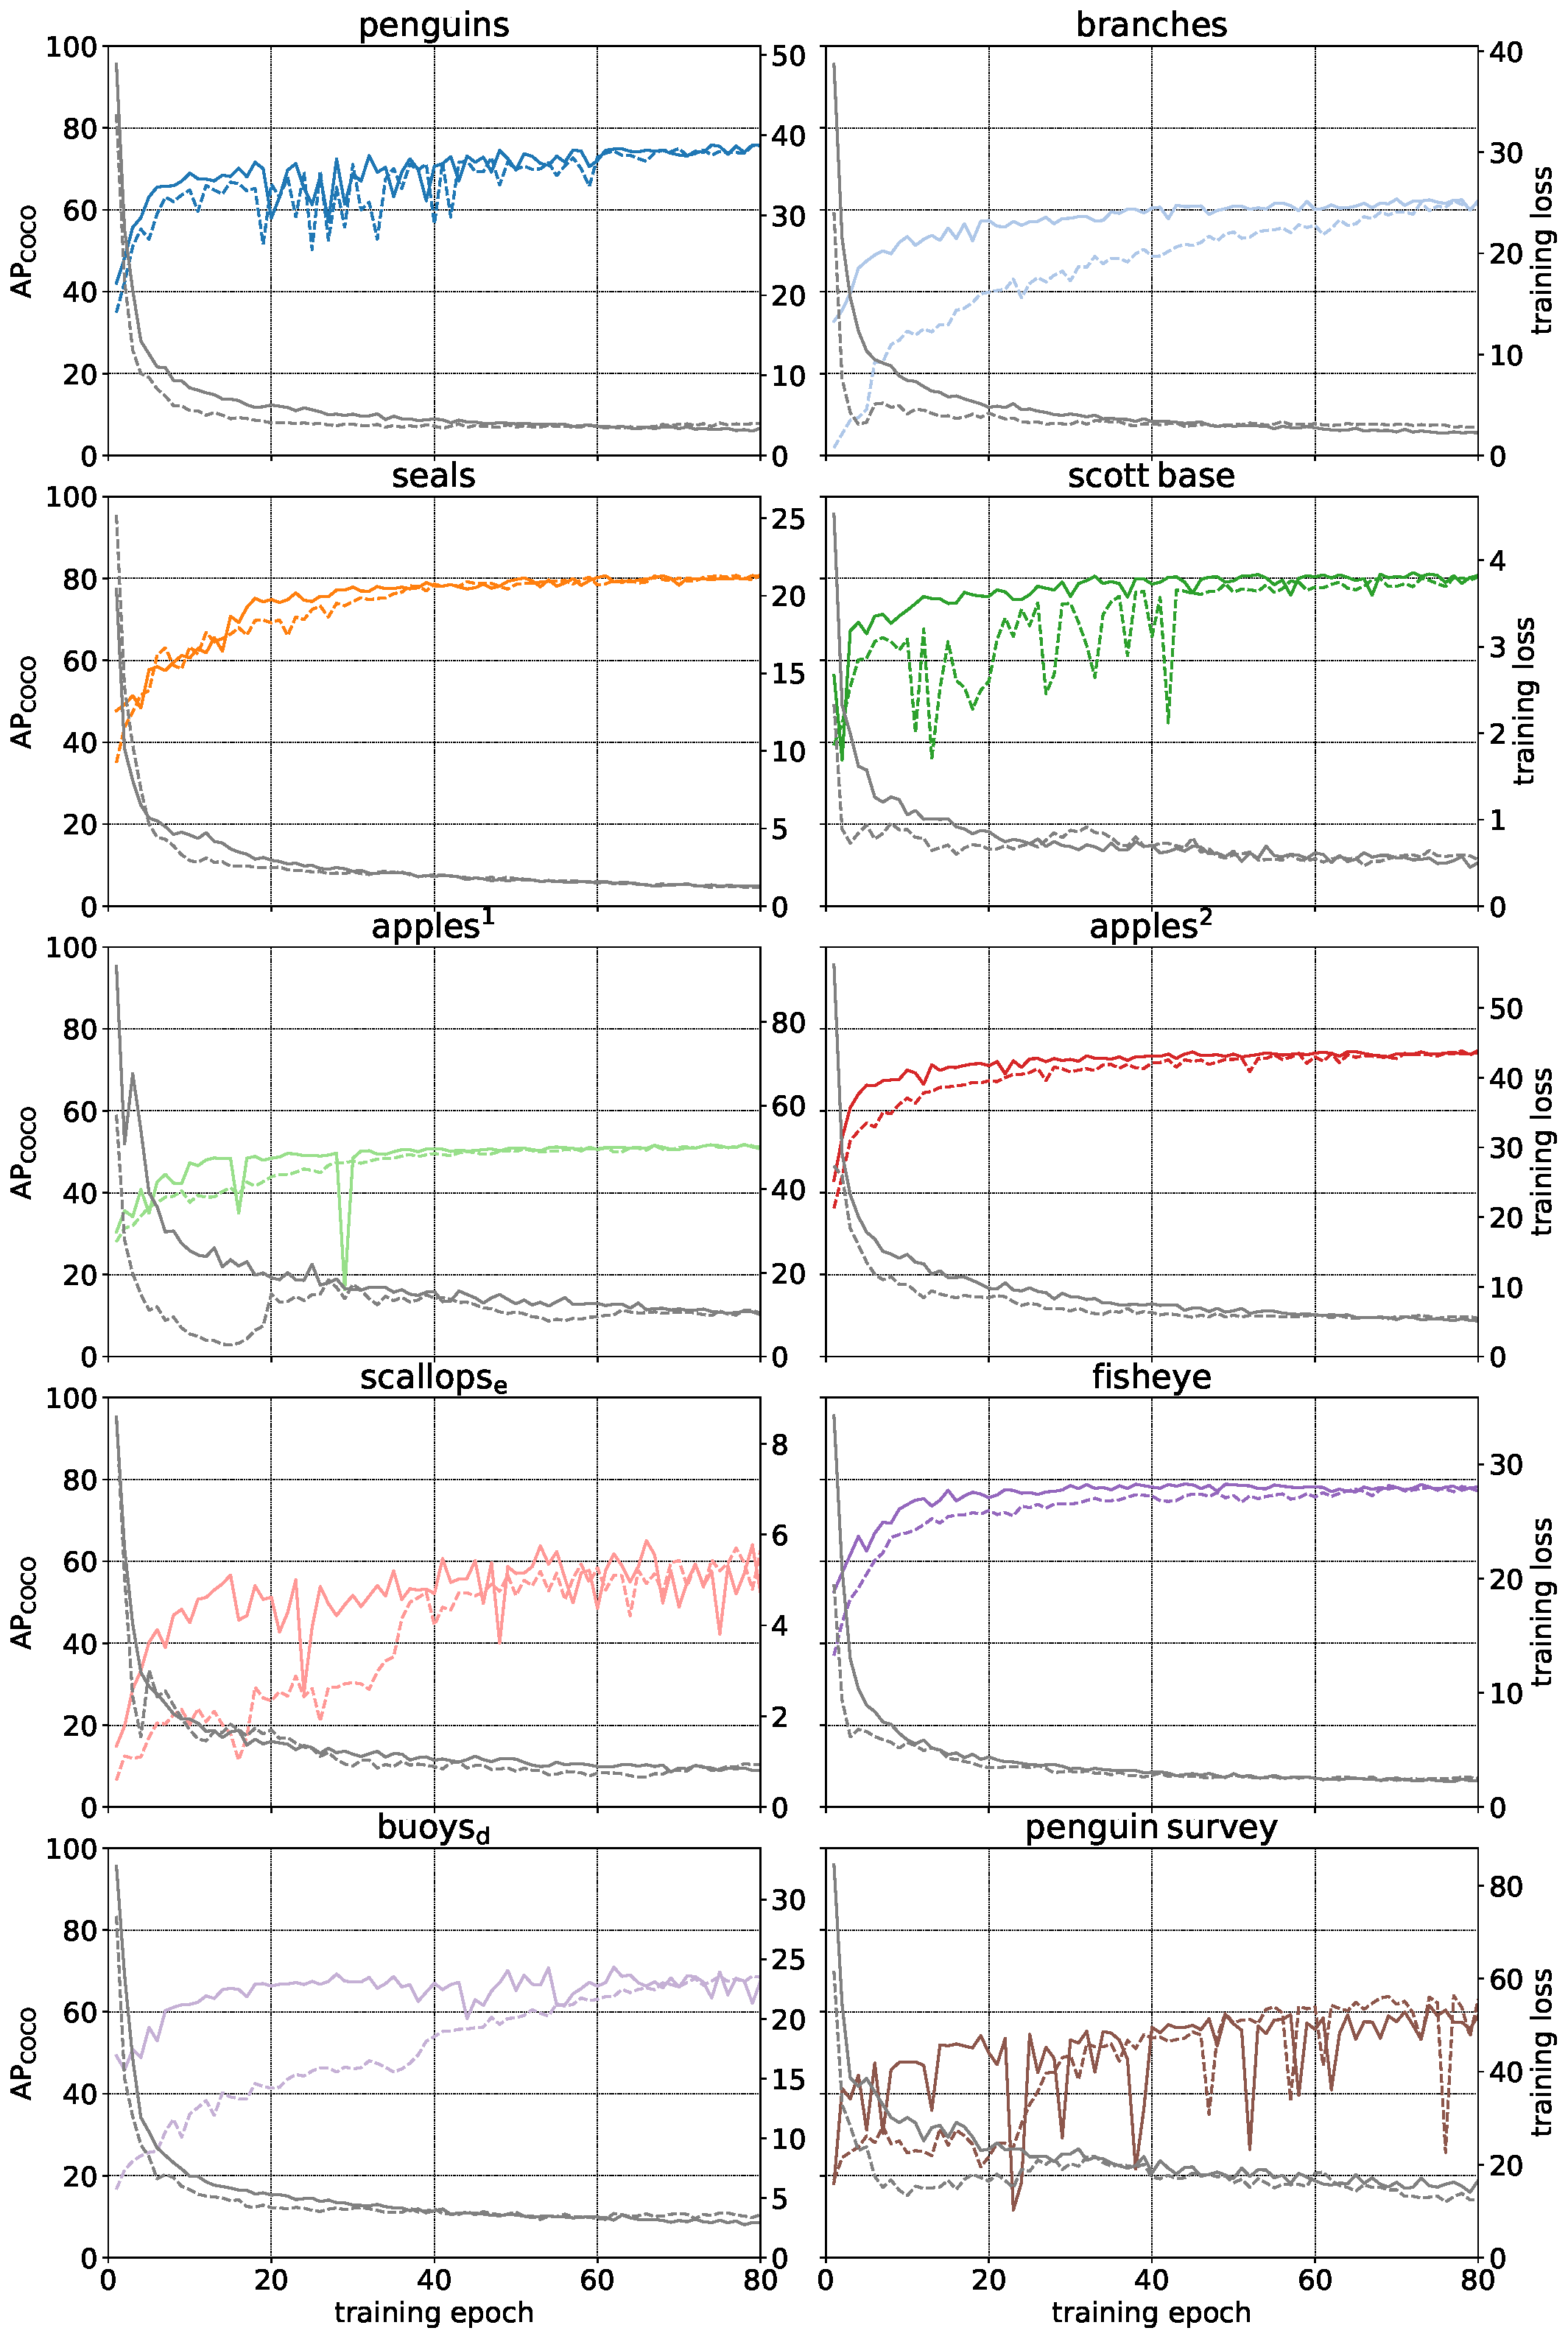
\includegraphics[width=1.0\linewidth]{figures/incremental.pdf}
  \caption{Incrementally adding examples vs. training with all examples from the beginning. Dotted lines are incremental training, solid lines are training with all examples up front. Grey lines at the bottom of each chart show the training loss.}  
  \label{fig:incremental}
\end{figure}

When using the annotation tool, image annotations become available incrementally. Here we investigate the difference between training with all examples annotated upfront compared to training with images added to the training set incrementally. 

During annotation, the validation set is incrementally built. Here we test against the final validation sets. In future, it would be better to use cross-validation, to make better use of training data, and provide more accurate testing (at the expense of extra training time). 

Figure~\ref{fig:incremental} shows the training plot for each dataset, where the validation accuracy ($AP_{COCO}$) is plotted against training time for both \emph{incremental} and \emph{full} cases. Different datasets improve at different rates with more data. However, all are restricted by the dataset size and improve with more data.



\section{Effect of localisation noise}


In this experiment, we examine how tolerant the object detector is to two factors: (a) random noisy annotations, (b) systematic bias and combinations of the two. All human annotation contains a certain amount of noise as well as a bias which varies from person to person and activity to activity, so it is expected an object detector can tolerate a certain amount of labelling noise in its training data. 

A \gls{VBA} based system by nature of using an object detector trained on noisy inputs, will therefore not produce entirely accurate localised predictions. The hope is that such a system will eventually produce localisations that are \emph{good enough} so that predictions from the object detector can be accepted without taking up valuable annotator time. In this experiment, we aim to quantify how noise degrades performance, and therefore establish some idea of what guideline for the level of precision is required during annotation.

\begin{figure}[!h]
\centering
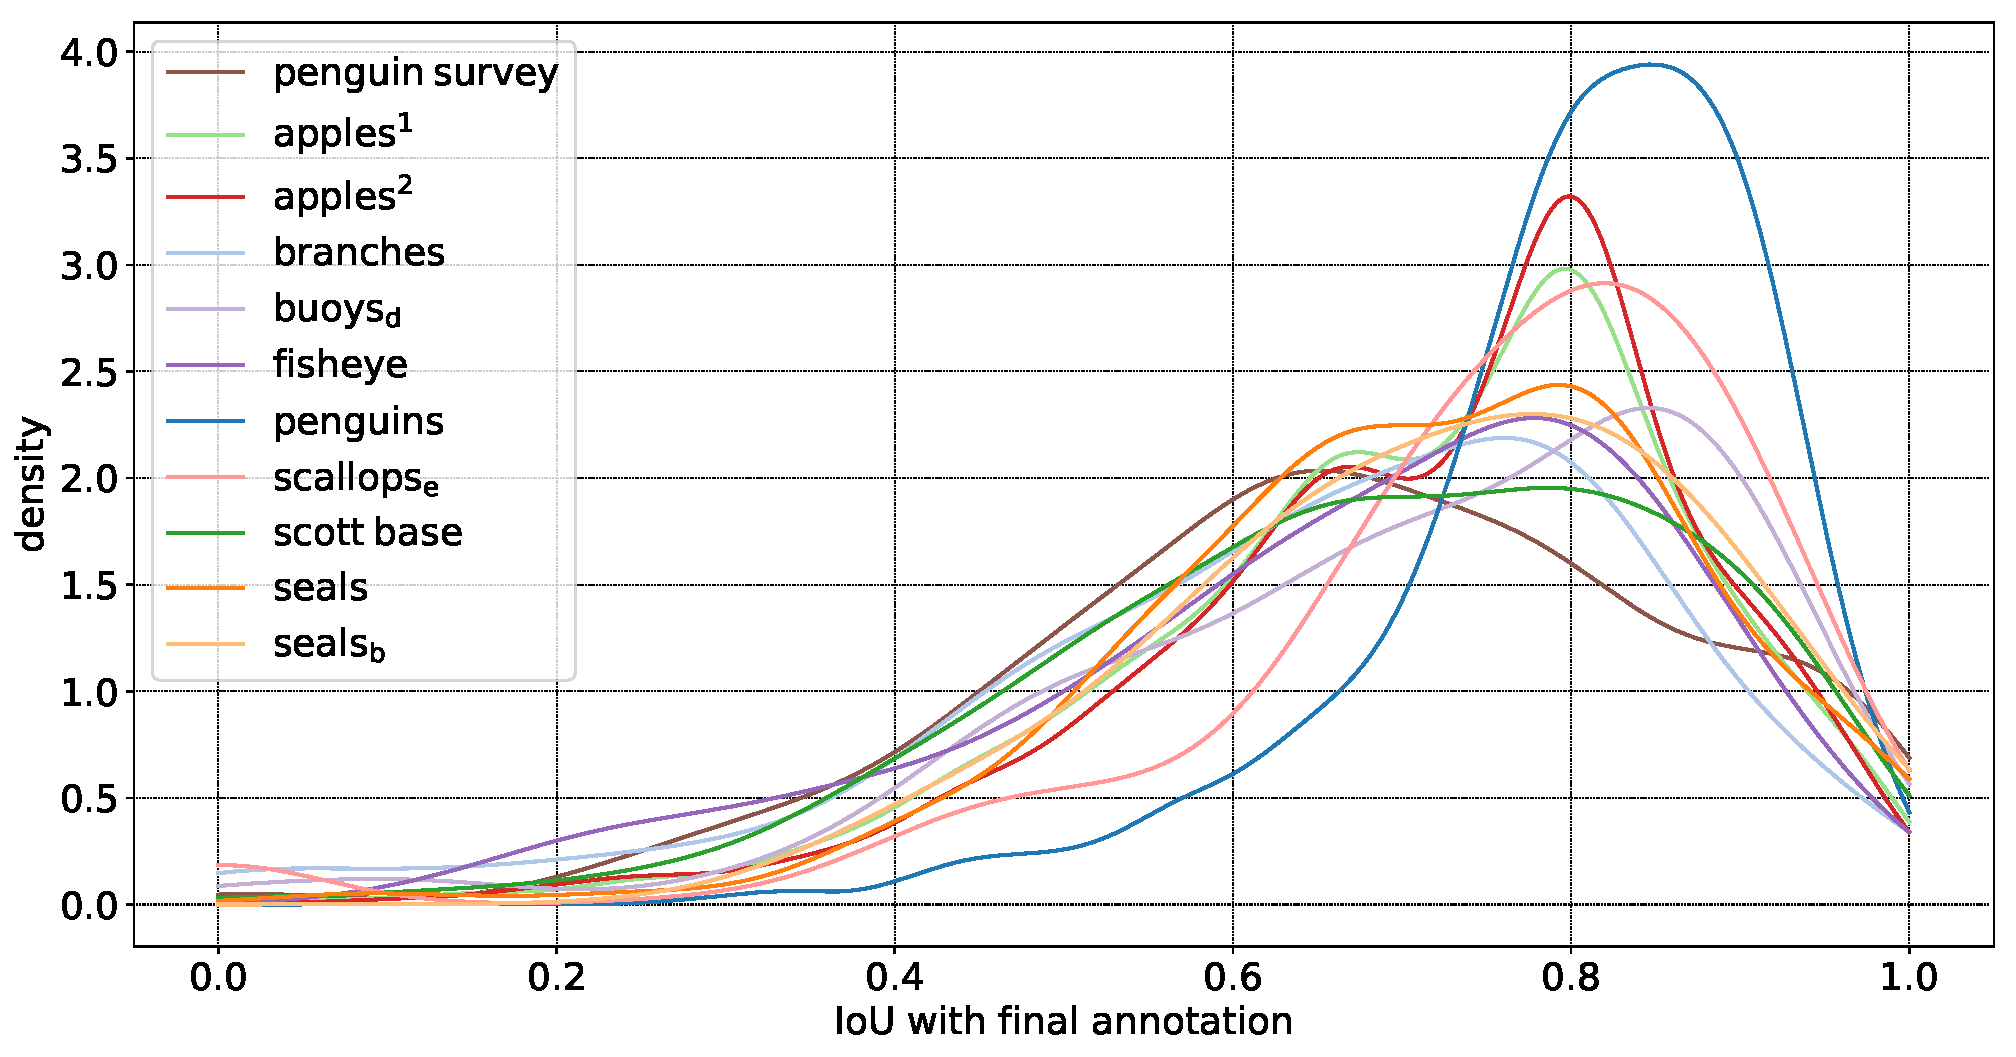
\includegraphics[width=1.0\linewidth]{figures/iou_dataset.pdf}
\caption{ Density plot of IoU overlap for detection with respect to annotation, for transformed detections. }
\label{fig:density_iou}
\end{figure}


\subsection {Human threshold}


Figure~\ref{fig:density_iou} shows in more detail the distribution of \gls{IOU} overlap for detections which have been modified. The density of transformed detections peaks at around $0.80$--$0.85$ depending on the dataset. It can be reasonably assumed that the real accuracy of the detections, which are used unmodified, would lie between that peak and $1.0$. Human annotation also has some degree of variability (reference \cite{Papadopoulos2017} gave a mean \gls{IOU} overlap of 88 for a box input method with Pascal VOC ground truth).

One minus the peak density seems like a reasonable surrogate measure for the human verification threshold. From the datasets annotated in this thesis the \emph{penguins} dataset annotation has the lowest threshold, at approximately $0.15$, and as a result, it seems likely the most precise localisation. For the \emph{penguin survey} the threshold is highest at around $0.35$. This makes sense because counting was emphasised as opposed to precise annotation, so, the localisation threshold is higher. 


\subsection{Method}

We added noise and systematic bias to five different datasets, covering a range of parameters (resolutions, object sizes, instance counts), where validation accuracy was highest among the datasets created in this work. These five are: \emph{branches}, $apples^2$ ($50\%$ scale), \emph{scott base}, \emph{seals} ($50\%$ scale) and \emph{penguins} ($50\%$ scale). Three datasets are down-sampled to save time. Two datasets are not down-sampled: one of them because the resolution is already low, and the other because the objects are already very small for the object detector.

Noise is added by randomly moving the box centre and randomly scaling the box size. The box centre ($c_x$, $c_y$) is moved as a proportion of the size of the box to become ($\hat{c}_x$, $\hat{c}_y$), and the width and height ($w$ and $h$) of the box are multiplied by translation ($t_x$, $t_y$) and scaling ($s_x$, $s_y$) factors sampled from a normal distribution. The standard deviation of the distribution $\sigma$ controls the magnitude of the translation and scaling. 

Systematic bias is added as a proportion of box width and height also, controlled by a parameter factor $\Delta$; in this experiment, the box is always moved up and to the right. The final transformed box is then specified by $\hat{c}_x$, $\hat{c}_y$, $\hat{w}$, $\hat{h}$ according to equation~\ref{eq:noisy_box}. 

\begin{equation}
\begin{split}
    s_w, s_h \sim \mathcal{N}(1,\,\sigma^{2})\\
    t_x, t_y \sim \mathcal{N}(0,\,\sigma^{2})\\
    \hat{c}_x = c_x + (\Delta + t_x) w\\
    \hat{c}_y = c_y + (\Delta + t_y) h\\
    \hat{w} = s_x w\\
    \hat{h} = s_h h\\
\end{split}
\label{eq:noisy_box}
\end{equation}

The noise is consistent throughout training as opposed to being added as a form of data label augmentation. Systematic offset factor $\Delta$ is also added to the validation set, assuming such a form of error would be uniform across the data. With an offset, the challenge for the object detector is if the detector can adapt its estimations when the real object in question is translated with respect to the centres in the feature map of the receptive field. Noise, on the other hand, is added only to the training data and not to the validation data as adding noise changes the mean of box centre or size (on average).

The object detector is trained for $40$ epochs in five different configurations of noise and systematic offset: $\sigma \in [0\%, 4\%, 8\%, 16\%, 32\%]$ and $\Delta \in [0\%, 4\%, 8\%, 16\%, 32\%]$. Object detectors are trained with standard parameters for each dataset (except the three which are trained at $50\%$ scale), and the impact of the noise and systematic offset is measured by looking at the peak validation \gls{AP} at different thresholds.

After noticing overfitting occurring in noisy cases, the set of experiments were repeated with reduced training data to examine how noise affected generalisation. We used two low training data scenarios, firstly at $25\%$ of training examples, then at $6.25\%$.

The amount of noise and the resulting mean \gls{IOU}s with the original box can be seen visually in Figure~\ref{fig:noisy_training}. It can be seen that the levels of noise and systematic offset, both have approximately the same mean \gls{IOU}s with respect to the original boxes for the particular level of offset or bias.

\begin{figure}[ht]
\centering
\begin{subfigure}[t]{0.5\linewidth}
  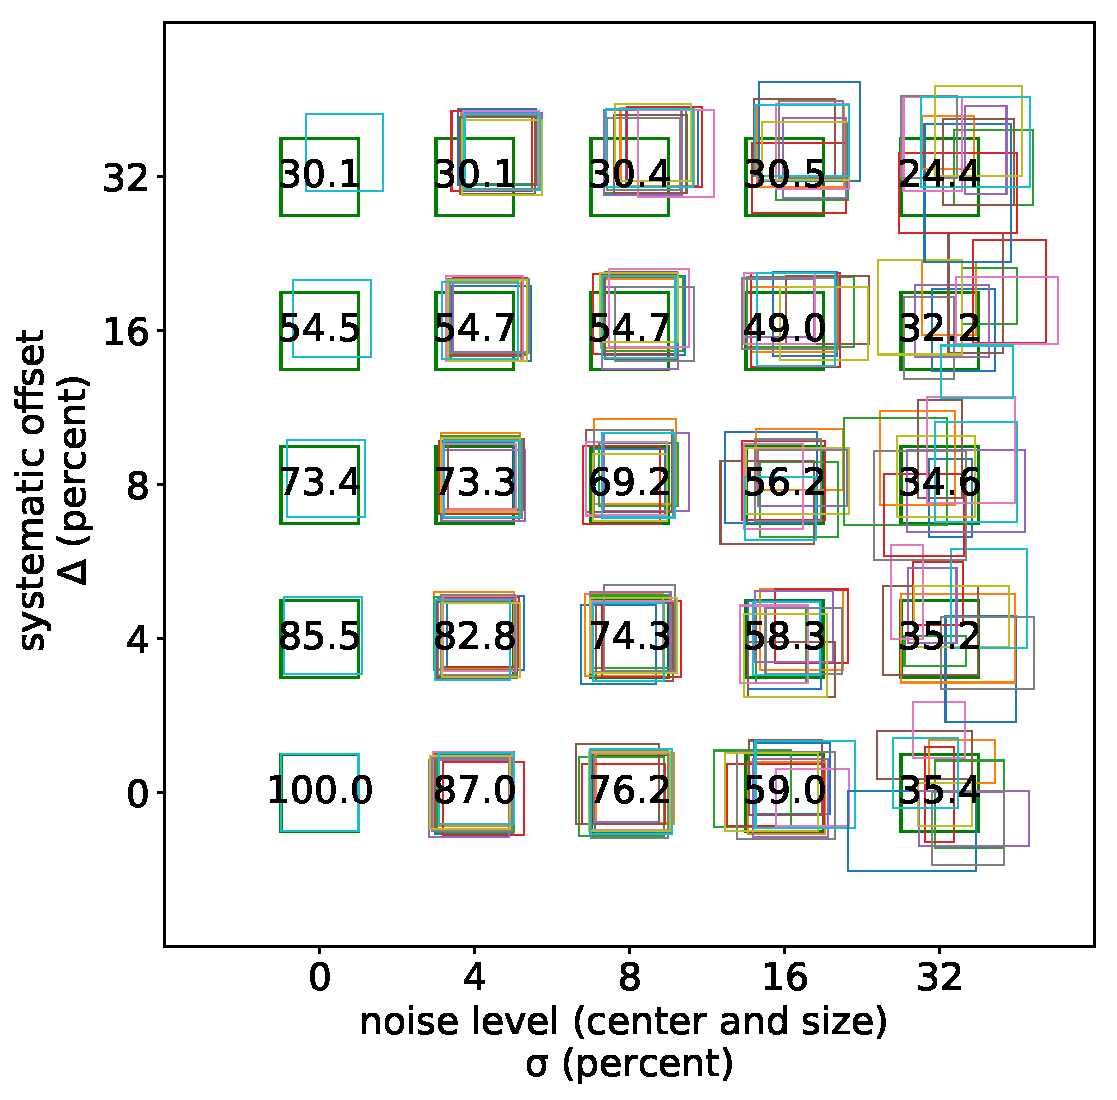
\includegraphics[width=1.0\linewidth]{figures/noisy_boxes.pdf}
  \caption{}
\end{subfigure}%
\begin{subfigure}[t]{0.5\linewidth}
  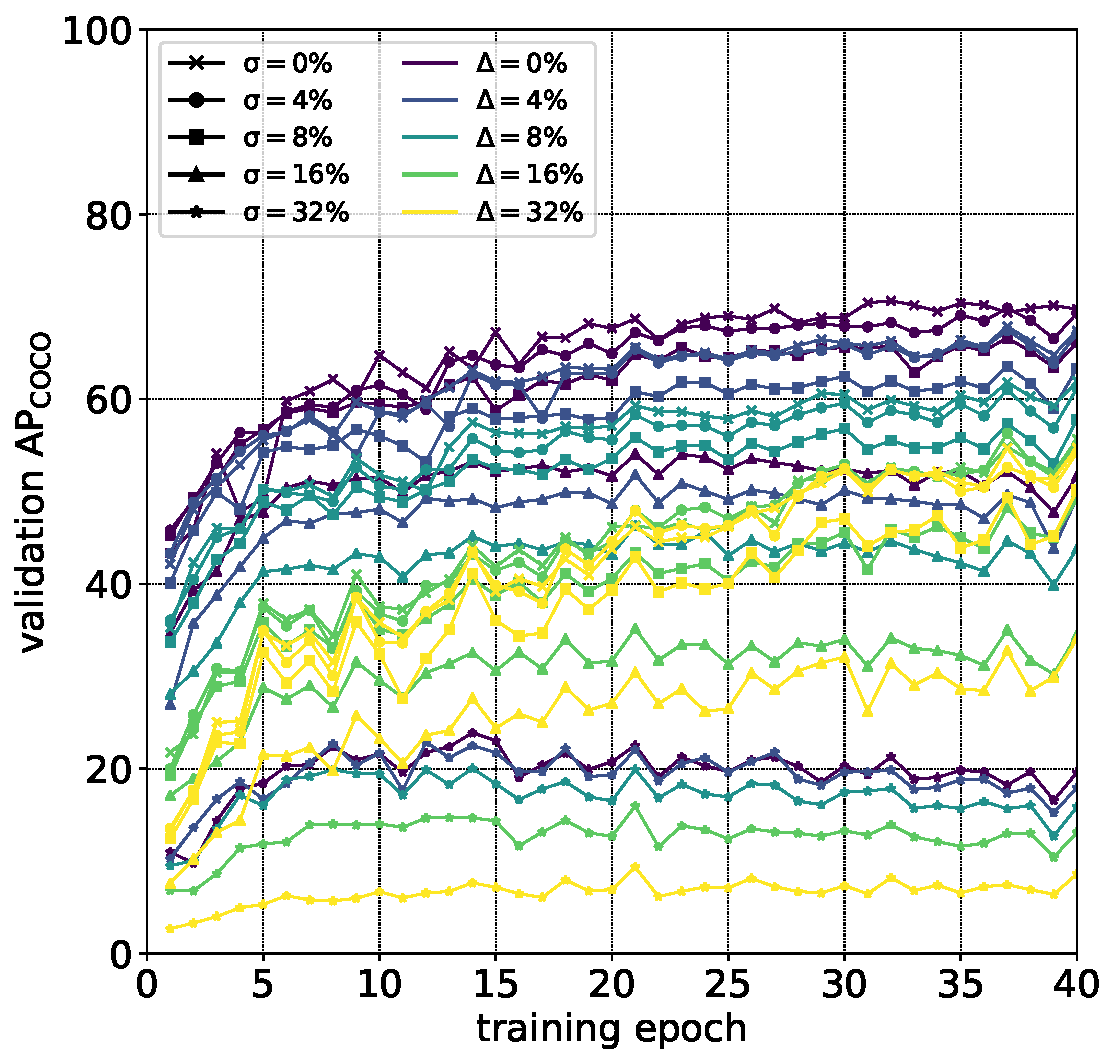
\includegraphics[width=1.0\linewidth]{figures/noise_training.pdf}
  \caption{100\% training images}
\end{subfigure}
\begin{subfigure}[t]{0.5\linewidth}
  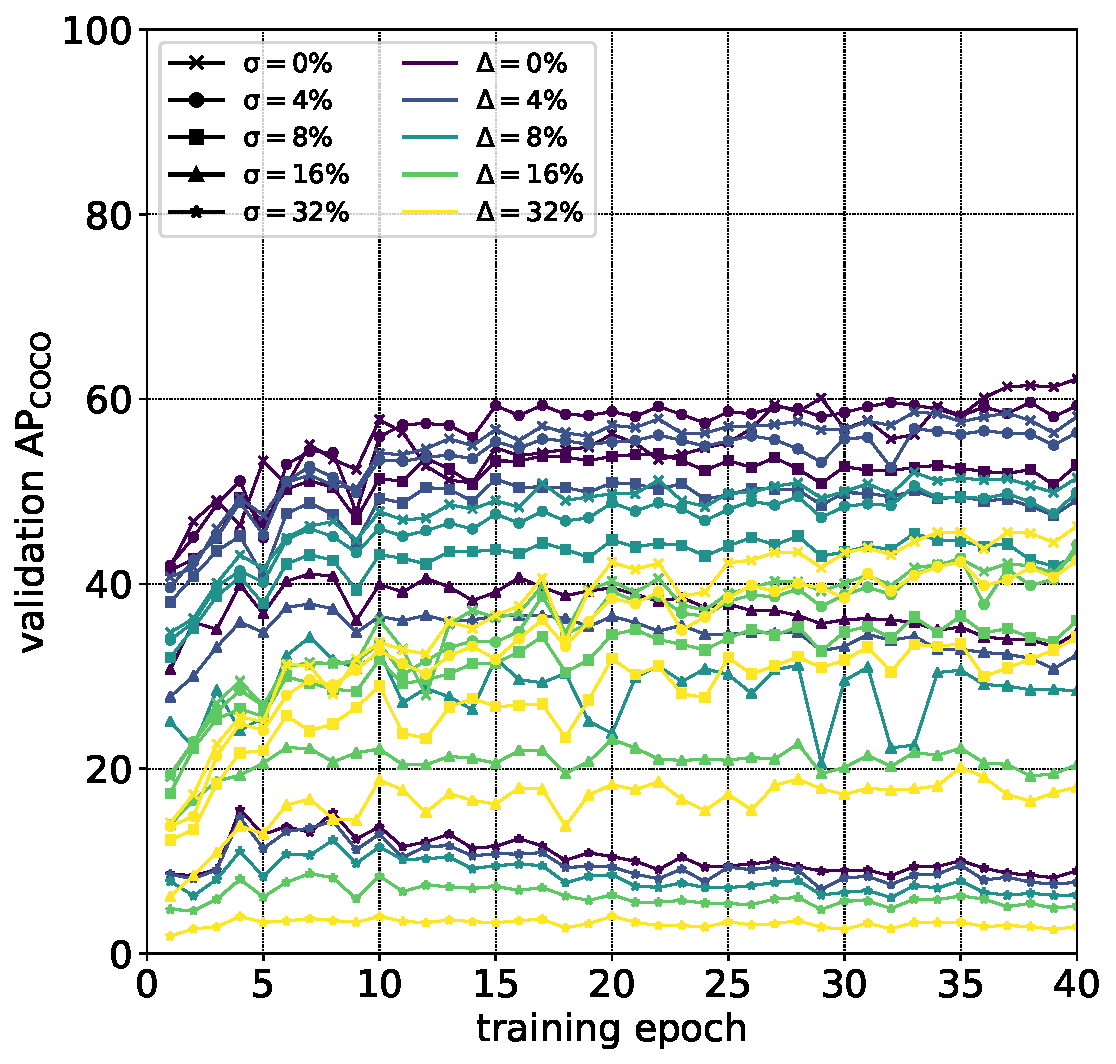
\includegraphics[width=1.0\linewidth]{figures/noise_4_training.pdf}
  \caption{25\% training images}
\end{subfigure}%
\begin{subfigure}[t]{0.5\linewidth}
  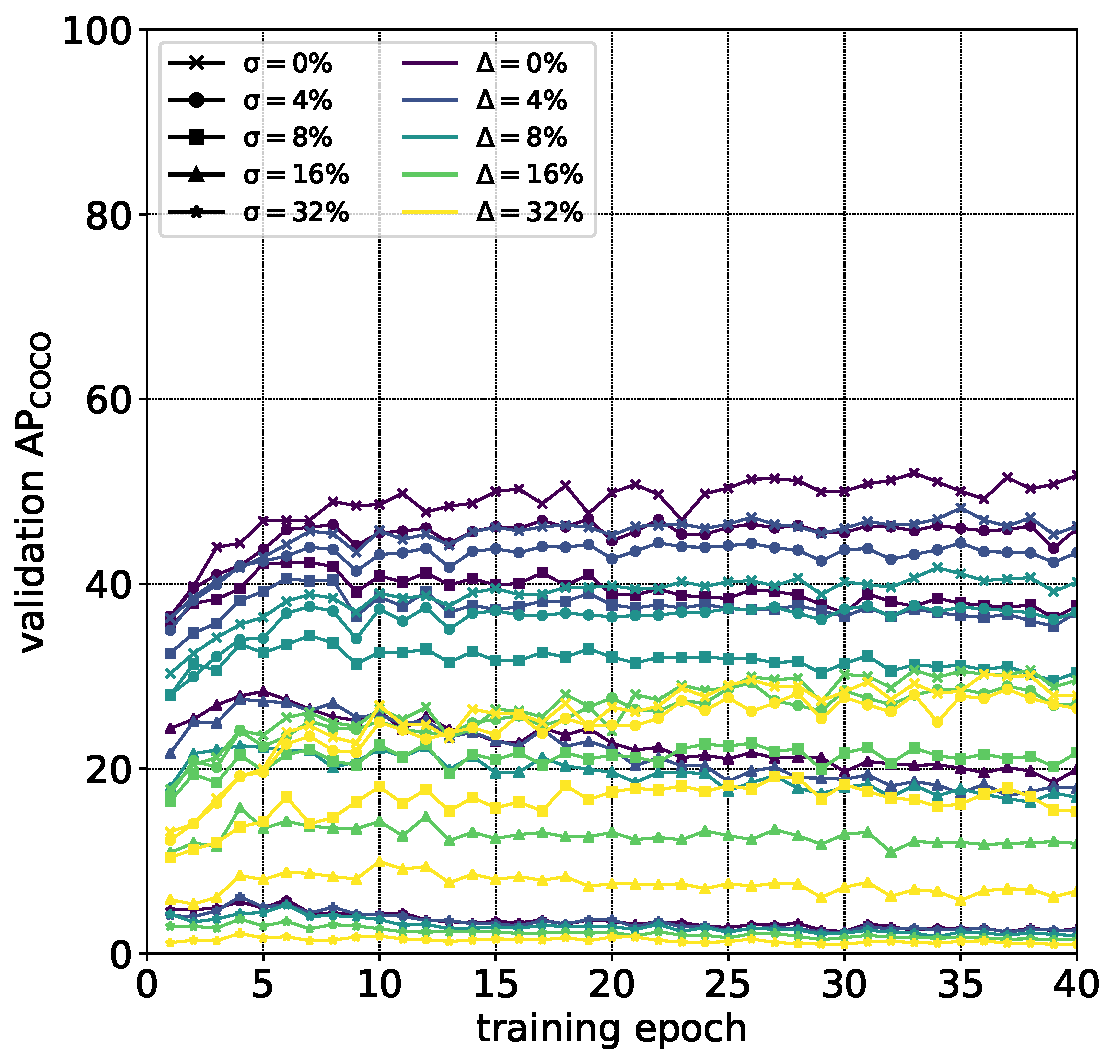
\includegraphics[width=1.0\linewidth]{figures/noise_16_training.pdf}
  \caption{6.25\% training images}
\end{subfigure}
  \caption{ (a) Samples of the different noise and systematic bias added, showing reference box with 10 samples; overlaid with the mean \gls{IOU} for that condition. (b), (c), (d) $AP_{COCO}$ validation after training with with varying noise and systematic bias added, and varying training set size. Average of training runs of 5 different datasets, at half-resolution: \emph{seals}, $apples^2$ and \emph{penguins}; at full-resolution: \emph{scott base}, \emph{branches}}
  \label{fig:noisy_training}
\end{figure}


\begin{table}[]
\caption {Best validation $AP_{50}$, $AP_{75}$, with different levels of added noise ($\sigma$) and systematic bounding box offset ($\Delta$) and at different sizes of training data. Baseline ($\sigma=0$, $\Delta=0$) in each case shown as absolute value in bold, other cases shown as percent change. Mean and standard deviation of 5 different datasets, at half-resolution: \emph{seals}, $apples^2$ and \emph{penguins}; at full-resolution: \emph{scott base}, \emph{branches}.}
\label{tab:noise_table}


\begin{subfigure}[b]{\linewidth}
\caption{$100\%$ training data}
\begin{adjustbox}{max width=\textwidth}
\begin{tabular}{ll|lllll}
 & & $\Delta=0\%$              & $\Delta=4\%$              & $\Delta=8\%$              & $\Delta=16\%$              & $\Delta=32\%$              \\

\toprule
\multirow{2}{*}{\STAB{\rotatebox[origin=c]{90}{$AP_{50}$}}}
 & $\sigma=0\%$  & $\mathbf{95.1\pm2.7}$  & $-0.6\pm0.6\%$  & $-0.7\pm0.7\%$  & $-2.8\pm2.1\%$  & $-10.1\pm10.6\%$ \\
 & $\sigma=4\%$  & $-0.3\pm0.6\%$  & $-0.4\pm0.6\%$  & $-1.3\pm1.4\%$  & $-2.8\pm1.7\%$  & $-10.4\pm10.3\%$ \\
 & $\sigma=8\%$  & $-1.1\pm0.8\%$  & $-1.3\pm1.7\%$  & $-2.4\pm1.5\%$  & $-4.0\pm2.3\%$  & $-12.6\pm9.8\%$  \\
 & $\sigma=16\%$ & $-6.9\pm4.7\%$  & $-8.4\pm5.3\%$  & $-8.0\pm4.4\%$  & $-10.2\pm3.7\%$ & $-23.8\pm11.7\%$ \\
 & $\sigma=32\%$ & $-32.6\pm6.8\%$ & $-32.1\pm7.1\%$ & $-36.1\pm4.4\%$ & $-42.2\pm4.8\%$ & $-61.5\pm6.6\%$ \\

\toprule
\multirow{2}{*}{\STAB{\rotatebox[origin=c]{90}{$AP_{75}$}}}
 & $\sigma=0\%$  & $\mathbf{84.0\pm8.5}$   & $-2.7\pm1.5\%$   & $-9.1\pm3.4\%$   & $-27.3\pm21.5\%$ & $-24.1\pm17.0\%$ \\
 & $\sigma=4\%$  & $-2.1\pm1.1\%$   & $-2.9\pm1.1\%$   & $-10.5\pm4.0\%$  & $-26.8\pm21.0\%$ & $-24.3\pm15.8\%$ \\
 & $\sigma=8\%$  & $-7.5\pm7.7\%$   & $-8.6\pm5.2\%$   & $-17.0\pm7.7\%$  & $-42.5\pm14.9\%$ & $-32.7\pm12.7\%$ \\
 & $\sigma=16\%$ & $-23.8\pm16.4\%$ & $-30.1\pm16.7\%$ & $-42.4\pm14.3\%$ & $-71.0\pm8.9\%$  & $-63.4\pm11.7\%$ \\
 & $\sigma=32\%$ & $-81.3\pm7.2\%$  & $-83.4\pm6.0\%$  & $-86.6\pm3.2\%$  & $-94.9\pm2.5\%$  & $-97.0\pm1.3\%$  \\
\bottomrule
\end{tabular}
\end{adjustbox}
\label{tab:noise_table_100}
\end{subfigure}
\begin{subfigure}[b]{\linewidth}
\caption{$25\%$ training data}
\begin{adjustbox}{max width=\textwidth}
\begin{tabular}{ll|lllll}
 & & $\Delta=0\%$              & $\Delta=4\%$              & $\Delta=8\%$              & $\Delta=16\%$              & $\Delta=32\%$              \\

\toprule
\multirow{2}{*}{\STAB{\rotatebox[origin=c]{90}{$AP_{50}$}}}
& $\sigma=0\%$ & $\mathbf{ 86.9\pm7.7 }$ & $-0.4\pm1.4\%$ & $-2.0\pm1.7\%$ & $-7.2\pm6.2\%$ & $-18.3\pm16.5\%$ \\ 
& $\sigma=4\%$ & $0.4\pm2.6\%$ & $0.5\pm1.5\%$ & $-1.6\pm2.5\%$ & $-8.1\pm7.4\%$ & $-19.8\pm14.8\%$ \\ 
& $\sigma=8\%$ & $-1.2\pm1.3\%$ & $-1.9\pm1.7\%$ & $-3.1\pm2.7\%$ & $-9.1\pm7.6\%$ & $-23.1\pm16.7\%$ \\ 
& $\sigma=16\%$ & $-9.0\pm7.7\%$ & $-9.2\pm6.6\%$ & $-11.9\pm9.1\%$ & $-20.4\pm10.9\%$ & $-38.3\pm12.6\%$ \\ 
& $\sigma=32\%$ & $-41.3\pm8.6\%$ & $-43.5\pm7.8\%$ & $-46.3\pm8.1\%$ & $-55.8\pm7.1\%$ & $-75.6\pm3.8\%$ \\ 


\toprule
\multirow{2}{*}{\STAB{\rotatebox[origin=c]{90}{$AP_{75}$}}}
& $\sigma=0\%$ & $\mathbf{ 72.8\pm16.4 }$ & $-6.3\pm6.4\%$ & $-18.6\pm9.0\%$ & $-39.5\pm17.5\%$ & $-29.2\pm19.2\%$ \\ 
& $\sigma=4\%$ & $-6.1\pm5.0\%$ & $-8.7\pm7.4\%$ & $-24.7\pm11.6\%$ & $-38.2\pm20.8\%$ & $-34.8\pm17.6\%$ \\ 
& $\sigma=8\%$ & $-19.1\pm17.8\%$ & $-21.7\pm14.8\%$ & $-33.2\pm14.7\%$ & $-56.3\pm14.8\%$ & $-51.1\pm18.9\%$ \\ 
& $\sigma=16\%$ & $-39.5\pm24.5\%$ & $-48.3\pm24.8\%$ & $-59.3\pm19.5\%$ & $-82.8\pm12.6\%$ & $-76.1\pm15.3\%$ \\ 
& $\sigma=32\%$ & $-86.9\pm7.9\%$ & $-87.2\pm9.1\%$ & $-92.3\pm5.5\%$ & $-97.6\pm1.4\%$ & $-98.7\pm0.5\%$ \\ 
\bottomrule
\end{tabular}
\end{adjustbox}
\label{tab:noise_table_4}
\end{subfigure}
\begin{subfigure}[b]{\linewidth}
\caption{$6.25\%$ training data}
\begin{adjustbox}{max width=\textwidth}
\begin{tabular}{ll|lllll}
 & & $\Delta=0\%$              & $\Delta=4\%$              & $\Delta=8\%$              & $\Delta=16\%$              & $\Delta=32\%$              \\

\toprule
\multirow{2}{*}{\STAB{\rotatebox[origin=c]{90}{$AP_{50}$}}}
& $\sigma=0\%$ & $\mathbf{ 75.1\pm23.2 }$ & $-3.9\pm7.7\%$ & $-4.2\pm6.5\%$ & $-15.4\pm11.8\%$ & $-31.7\pm19.6\%$ \\ 
& $\sigma=4\%$ & $-6.7\pm9.9\%$ & $-2.1\pm3.2\%$ & $-4.0\pm2.0\%$ & $-15.7\pm14.1\%$ & $-31.6\pm19.8\%$ \\ 
& $\sigma=8\%$ & $-2.2\pm2.7\%$ & $-4.6\pm6.1\%$ & $-8.8\pm9.1\%$ & $-18.9\pm10.1\%$ & $-42.8\pm17.6\%$ \\ 
& $\sigma=16\%$ & $-18.7\pm9.8\%$ & $-21.0\pm15.5\%$ & $-21.9\pm8.3\%$ & $-30.2\pm11.6\%$ & $-58.8\pm12.7\%$ \\ 
& $\sigma=32\%$ & $-68.6\pm12.2\%$ & $-70.8\pm10.6\%$ & $-71.6\pm8.4\%$ & $-76.6\pm9.0\%$ & $-87.1\pm5.3\%$ \\ 

\toprule
\multirow{2}{*}{\STAB{\rotatebox[origin=c]{90}{$AP_{75}$}}}
& $\sigma=0\%$ & $\mathbf{ 61.5\pm26.7 }$ & $-8.8\pm6.4\%$ & $-29.3\pm9.8\%$ & $-55.1\pm13.6\%$ & $-46.9\pm14.1\%$ \\ 
& $\sigma=4\%$ & $-10.1\pm5.0\%$ & $-16.7\pm8.9\%$ & $-40.6\pm14.1\%$ & $-58.7\pm19.1\%$ & $-51.8\pm14.4\%$ \\ 
& $\sigma=8\%$ & $-25.7\pm15.2\%$ & $-32.9\pm18.1\%$ & $-51.4\pm12.9\%$ & $-76.8\pm10.9\%$ & $-76.5\pm6.7\%$ \\ 
& $\sigma=16\%$ & $-63.7\pm20.6\%$ & $-67.9\pm23.2\%$ & $-77.0\pm15.2\%$ & $-92.4\pm7.7\%$ & $-93.4\pm5.1\%$ \\ 
& $\sigma=32\%$ & $-97.4\pm1.8\%$ & $-97.2\pm1.8\%$ & $-98.0\pm1.2\%$ & $-98.7\pm0.7\%$ & $-99.6\pm0.2\%$ \\ 

\bottomrule
\end{tabular}
\end{adjustbox}
\label{tab:noise_table_16}
\end{subfigure}
\end{table}


The impact in terms of degradation of object detection performance can be seen in Table~\ref{tab:noise_table}, shown as the reduction in performance from the baseline zero noise and zero offset cases (shown as the absolute value, in bold). Two matching thresholds are shown, a relaxed matching threshold $AP_{50}$ and at strict matching threshold $AP_{75}$. 

The object detector at a relaxed matching threshold $AP_{50}$ is robust to a small amount of noise and systematic offset; less than $8\%$ offset or noise shows only a small impact on $AP_{50}$ degradation in each case, even in the low data scenarios. For the full amount of data, $AP_{50}$ is only degraded $10\%$ at $\sigma = 16\%, \Delta = 16\%$, yet in the same case $AP_{75}$ is reduced by $71\%$.

For the full amount of training data, $AP_{75}$ is also robust to a small amount of noise or offset, roughly $2\%$ degradation of performance for $4\%$ noise or offset. Human variation of box annotation in \cite{Papadopoulos2017} was reported as a mean \gls{IOU} of 88, which corresponds to the noise case of $\sigma = 4\%$. At that noise level, performance degradation is minimal, even for a strict matching criterion, degrading $AP_{75}$ by around $2\%$. Keep in mind that these datasets were human-annotated to begin with, so the noise added is extra noise.

Sensitivity to noise and systematic offset is seen to increase significantly with less training data. At $\sigma=4\%$, a level of noise similar to a human annotator, $AP_{75}$ is degraded by $2.1\%$ at $100\%$ images, increasing to $6.1\%$ at $25\%$ images and $10.1\%$ at $6.25\%$ of the training images. This increased sensitivity can be seen across the range of noise and offset, and at $6.25\%$ of the images, $AP_{50}$ is degraded approximately double the amount compared to at $25\%$ of the images.


\section {Conclusions}

We presented our approach to object detection for Verification Based Annotation, where (with a few minor changes) an object detector \cite{Lin2017} can be robust, without a large degree of parameter tweaking, for object detection in a wide variety of domains with a variety of image resolution and object size.

By training with image crops, higher accuracy is possible using the full image resolution (at the expense of training time, however during annotation, time is plentiful). In each case, using larger crop sizes proved better, more accurate and more stable. Two high-resolution inference methods were approximately equal, with the tiling approach allowing larger images at the expense of inference time. Incremental training was shown to be practical, with different datasets scaling in accuracy (and in time required for training) differently with the addition of extra images. 

An investigation of the impact of annotation localisation noise and systematic error on box annotation shows that training with many images is robust to a small amount of localisation error. However, with fewer images the sensitivity is much higher, leading to degradation of performance with even a small amount of noise; this suggests a focus on accurate object localisation is important, especially near the beginning of annotation, for both annotator and tool author.

\section*{Acknowledgment}

Thanks to Dr Regina Eisert for use of seal images ($\mathrm{seals}$, $\mathrm{scott\:base}$), Antarctica New Zealand for use of the aerial penguin survey images ($\mathrm{aerial\:survey}$) and Lincoln Agritech for apple dataset ($\mathrm{apples_2}$).

\bibliographystyle{unsrt}
\bibliography{references}

\end{document}